\NeedsTeXFormat{LaTeX2e}
%-----------------------------------------------------------
\documentclass[a4paper,12pt]{monografia}
\usepackage[portuguese, colorinlistoftodos, textsize=tiny]{todonotes}
\usepackage{amsmath,amsthm,amsfonts,amssymb}
\usepackage[mathcal]{eucal}
\usepackage{latexsym}
\usepackage[portuguese]{babel}  
\usepackage[utf8]{inputenc}
\usepackage{setspace}
%\usepackage{natbib}
\usepackage{bm}
\usepackage[portuguese,algoruled,longend, linesnumbered]{algorithm2e}
\usepackage{listings}
\usepackage{graphicx}
\usepackage{float}
\usepackage{booktabs}
\usepackage{hyperref}
\hypersetup{colorlinks,
   debug=false,
   linkcolor=black,  %%% cor do tableofcontents, \ref, \footnote, etc
   citecolor=black,  %%% cor do \cite
   urlcolor=black,   %%% cor do \url e \href
   bookmarksopen=true,
}
\usepackage[alf,bibjustif]{abntex2cite}

\usepackage{tikz}
\usetikzlibrary{arrows.meta, positioning}
\usetikzlibrary{shapes.geometric, fit, backgrounds}

\newcounter{todocounter}
\newcommand{\comment}[2][]
{\stepcounter{todocounter}\todo[caption={\thetodocounter: #2}, #1] 
{\begin{spacing}{1}\thetodocounter: #2\end{spacing}}}
\reversemarginpar
\setlength{\marginparwidth}{2.5cm}
\lstloadlanguages{C,SQL}
%-----------------------------------------------------------
%-----------------------------------------------------------
\theoremstyle{plain}
\newtheorem{theorem}{Teorema}[section]
\newtheorem{axiom}{Axioma}[section]
\newtheorem{corollary}{Corol\'ario}[section]
\newtheorem{lemma}{Lema}[section]
\newtheorem{proposition}{Proposi\c{c}\~ao}[section]
%-----------------------------------------------------------
\theoremstyle{definition}
\newtheorem{definition}{Defini\c{c}\~ao}[section]
\newtheorem{example}{Exemplo}[section]
%-----------------------------------------------------------
\theoremstyle{remark}
\newtheorem{remark}{Observa\c{c}\~ao}[section]
%-----------------------------------------------------------
%-----------------------------------------------------------
\newcommand{\R}{\mathbb{R}}
\newcommand{\N}{\mathbb{N}}
\newcommand{\Z}{\mathbb{Z}}
\newcommand{\Q}{\mathbb{Q}}
\newcommand{\K}{\mathbb{K}}
\newcommand{\I}{\mathbb{I}}
\newcommand{\id}{\mathbf{1}}
\newcommand{\U}{\mathcal{U}}
\newcommand{\V}{{\cal V}}
% --------------------------------------------------
\def\ind{\hbox{ ind }}
% --------------------------------------------------
\begin{document}
% --------------------------------------------------
\titulo{Data Warehouse para análise da execução orçamentária municipal}
% \subtitulo{Subtítulo (opcional)}
\autor{Antônio Marcos Souza Pereira}

% --------------------------------------------------
\bacharelado % Pode ser \bacharelado \licenciatura \especializacao \mestrado ou \doutorado
\curso{Ciência da Computação} 
\ano{2026}
\cidade{Juiz de Fora}

% --------------------------------------------------
\instituicao{Universidade Federal de Juiz de Fora} \sigla{UFJF}
\unidadeacademica{Instituto de Ciências Exatas}
\departamento{Departamento de Ciência da Computação}

% --------------------------------------------------
\orientador{Victor Ströele de Andrade Menezes}
\ttorientador{Doutor em Engenharia de Sistemas e Computação pela UFRJ}

% \coorientador{Nome do Co-orientador}
% \ttcoorientador{Título do Co-orientador}

\examinadorum{José Maria Nazar David}
\ttexaminadorum{Doutor em Engenharia de Sistemas e Computação pela UFRJ}

\examinadordois{Regina Maria Maciel Braga Villela}
\ttexaminadordois{Doutora em Engenharia de Sistemas e Computação pela UFRJ}

% \examinadortres{Nome do Examinador 3}
% \ttexaminadortres{Título do Examinador 3}

% \examinadorquatro{Nome do Examinador 4}
% \ttexaminadorquatro{Título do Examinador 4}

% --------------------------------------------------
% \CDU{536.21} \areas{1.Análise Matemática  2. Topologia.}
% \npaginas{xx}
% \inserirlogo
\maketitle

% --------------------------------------------------
% \begin{dedicatoria}
% Pensar em uma dedicatória legal pra por aqui.
% \end{dedicatoria}


% --------------------------------------------------
\resumo{Resumo}
A divulgação de dados orçamentários municipais avançou com a ampliação dos Portais da Transparência, mas a forma como essas informações são disponibilizadas ainda impõe barreiras à compreensão da população. Planilhas extensas, formatos heterogêneos e linguagem técnica dificultam o acompanhamento efetivo da execução orçamentária e limitam o exercício do controle social. Este trabalho propõe e implementa um \textit{Data Warehouse} para análise da execução orçamentária de Juiz de Fora, integrando informações dispersas do Portal da Transparência municipal, do ementário da Secretaria do Tesouro Nacional e da Lei Orçamentária Anual em um modelo dimensional. A pesquisa adota \textit{Design Science Research} como abordagem metodológica e a modelagem dimensional de Kimball como referência técnica. O artefato resultante integra dez dimensões e três tabelas de fatos de despesas e receitas, alimentadas por um \textit{pipeline} de ETL idempotente que documenta explicitamente as inconsistências encontradas nas fontes. O consumo ocorre por meio de sete painéis interativos publicados em instância pública, avaliados comparativamente ao portal original em tarefas representativas de fiscalização. Os resultados mostram uma redução consistente do esforço de consolidação manual exigido do usuário e revelam padrões recorrentes na execução orçamentária municipal, entre eles a dependência de transferências intergovernamentais e a distância entre o empenho e o pagamento efetivo.

\vspace{0.3cm}
\noindent\textbf{Palavras-chave}: transparência pública; orçamento municipal; \textit{data warehouse}; modelagem dimensional; \textit{design science  research}; controle social.

\resumo{Abstract}
The disclosure of municipal budget data has advanced with the expansion of Transparency Portals, but the way this information is made available still imposes barriers to public understanding. Extensive spreadsheets, heterogeneous formats, and technical language hinder effective monitoring of budget execution and limit the exercise of social control. This work proposes and implements a Data Warehouse to analyze budget execution in Juiz de Fora, integrating dispersed information from the municipal Transparency Portal, the National Treasury Secretariat's revenue classification catalog, and the Annual Budget Law into a dimensional model. The research adopts Design Science Research as its methodological approach and Kimball's dimensional modeling as its technical reference. The resulting artifact integrates ten dimensions and three fact tables on expenditures and revenues, fed by an idempotent ETL pipeline that explicitly documents the inconsistencies found in the source data. Consumption is provided through seven interactive dashboards published on a public instance and evaluated against the original portal for representative fiscalization tasks. The results show a consistent reduction in the manual consolidation effort required of the user and reveal recurring patterns in municipal budget execution, including dependence on intergovernmental transfers and a gap between commitment and effective payment.

\vspace{0.3cm}
\noindent\textbf{Keywords}: public transparency; municipal budget; data warehouse; dimensional modeling; design science research; social control.

% --------------------------------------------------
\agradecimento{Agradecimentos} \indent\indent 
À minha mãe, por todos os sacrifícios que me trouxeram até aqui. À minha namorada e aos meus amigos, pela companhia e pelo apoio durante essa caminhada. Ao meu orientador, pelo apoio nesta monografia. A todos os funcionários do Departamento de Ciência da Computação da UFJF, que, de alguma forma, contribuíram com a minha formação até aqui. E ao povo brasileiro, que financiou cada dia desta graduação. Universidade pública, gratuita e de qualidade é conquista popular, e é dever de todos defendê-la.

\newpage

% --------------------------------------------------
\begin{epigrafe}
"A leitura do mundo precede a leitura da palavra".\\
\hfill Paulo Freire
\end{epigrafe}

% -----Sumário--------------------------------------
\tableofcontents \thispagestyle{empty} \listoffigures
\thispagestyle{empty} \listoftables \thispagestyle{empty}

% -----Glossário------------------------------------
\chapter*{Lista de Abreviações} \addcontentsline{toc}{chapter}{Lista de Abreviações}
\doublespacing  \begin{tabular}{l l}

API   & \textit{Application Programming Interface} \\
BI    & \textit{Business Intelligence} \\
CGU   & Controladoria-Geral da União \\
DCC   & Departamento de Ciência da Computação \\
DW    & \textit{Data Warehouse} \\
ETL   & \textit{Extract, Transform, Load} \\
LAI   & Lei de Acesso à Informação \\
LDO   & Lei de Diretrizes Orçamentárias \\
LOA   & Lei Orçamentária Anual \\
MCASP & Manual de Contabilidade Aplicada ao Setor Público \\
MTO   & Manual Técnico de Orçamento \\
OCR   & \textit{Optical Character Recognition} \\
PJF   & Prefeitura de Juiz de Fora \\
PPA   & Plano Plurianual \\
SCD   & \textit{Slowly Changing Dimension} \\
SQL   & \textit{Structured Query Language} \\
STN   & Secretaria do Tesouro Nacional \\
UFJF  & Universidade Federal de Juiz de Fora \\

\end{tabular}  \thispagestyle{empty}

% -----Conteúdo-------------------------------------
\pagestyle{ruledheader}
\chapter{Introdução}
\label{cap:intro}

A Lei de Acesso à Informação (LAI), promulgada em 2011, consolidou o direito do cidadão de obter dados produzidos pelo Estado brasileiro \cite{Lei:12.527:2011}. Como desdobramento dessa legislação, os portais municipais de transparência passaram a publicar informações sobre orçamento, finanças e administração. Publicar dados, por si só, não basta. A linguagem técnica do orçamento, a fragmentação das informações em múltiplas tabelas e a ausência de ferramentas de análise mantêm o cidadão distante da compreensão de como os recursos públicos são gastos \cite{matiaspereira2010,melo2019proposta}.

O Data Warehouse (DW) surge como resposta tecnológica a esse problema. Trata-se de um repositório que integra dados de fontes heterogêneas e os organiza para análise \cite{kimball2013data}. A modelagem dimensional, consolidada por \citeonline{kimball2013data}, prioriza a usabilidade da consulta em relação à otimização das transações. Em vez de planilhas que exigem do usuário cruzar referências manualmente, tabelas de fatos e dimensões permitem que perguntas relevantes sejam respondidas com poucos cliques: "Quanto Juiz de Fora investiu em educação nos últimos três anos?", "Qual o tempo médio de pagamento aos fornecedores da área de saúde?", "Há concentração de recursos em poucos favorecidos?". Essas perguntas, antes restritas a especialistas em finanças públicas, passam a ser acessíveis a jornalistas, conselheiros municipais e organizações da sociedade civil \cite{marco2022transparencia}.

A transparência orçamentária brasileira convive com um paradoxo. A base legal existe, os portais estão no ar, os dados são publicados. Mesmo assim, a participação cidadã na fiscalização do gasto público permanece restrita. A literatura aponta três lacunas que sustentam essa distância entre a disponibilidade formal e o uso real da informação: a lacuna social, a técnica e a pedagógica.

A lacuna social refere-se às barreiras ao letramento financeiro e digital. Cidadãos comuns têm dificuldade não só em acessar dados, mas também em relacioná-los à própria experiência. O orçamento público, apresentado em categorias contábeis como "elemento de despesa", "função programática" e "fonte de recurso", permanece distante da realidade da escola, do posto de saúde e da via pública. A opacidade técnica desmobiliza a participação e reforça o privilégio de quem tem formação especializada ou acesso a intermediários, como ONGs e jornalismo investigativo. O resultado é um déficit democrático: a transparência formal coexiste com a opacidade prática.

A lacuna técnica está nos próprios portais. Os dados costumam ser disponibilizados em formatos pouco amigáveis à análise, como PDFs sem estrutura ou planilhas sem padronização, e raramente há APIs ou recursos para o cruzamento de informações entre bases distintas (despesas, receitas, licitações). Quem deseja produzir análises temporais ou identificar padrões anômalos enfrenta um trabalho manual de coleta, limpeza e consolidação que poucos podem custear em termos de tempo e de especialização. O Data Warehouse altera essa equação ao consolidar o esforço analítico em uma estrutura reutilizável.

A lacuna pedagógica é a menos debatida e fundamenta-se na obra de Paulo Freire, em especial na noção de educação libertadora e no conceito de conscientização \cite{freire1967liberdade}. Freire argumenta que a transformação social depende da capacidade de "ler o mundo" criticamente, superando a passividade diante das estruturas de dominação. Aplicado ao orçamento público, isso significa que a democratização do poder vai além da publicação passiva de dados: exige instrumentos que capacitem o cidadão a formular perguntas, testar hipóteses e construir suas próprias leituras sobre a gestão pública \cite{freire1996autonomia}. O conceito freireano de "inédito viável" descreve com precisão o lugar do Data Warehouse civil. Trata-se de uma forma de participação ainda incipiente, em que o cidadão questiona não só quanto foi gasto, mas também por que aquela área recebeu mais recursos, se o investimento responde às necessidades locais e se há sinais de favorecimento a fornecedores específicos.

A escolha da execução orçamentária municipal como objeto de estudo não é arbitrária. É na esfera local que as políticas públicas ganham forma concreta no cotidiano dos moradores, e é onde o controle social direto encontra mais espaço \cite{novaes2014orcamento}. Ao documentar a construção de um DW para a gestão municipal, o trabalho oferece uma referência metodológica que outros municípios poderiam adaptar, sujeita aos ajustes específicos de parsing de cada portal. O recorte também preenche uma lacuna específica na interdisciplinaridade. Estudos sobre transparência pública costumam permanecer no terreno da análise política ou jurídica. Estudos sobre DW raramente discutem implicações cívicas. Esse trabalho se posiciona no encontro entre as duas e sustenta uma tese: a arquitetura de dados é uma escolha política, pois define quem pode participar do debate público e em que termos.

Metodologicamente, o trabalho adota \textit{Design Science Research} (DSR) como abordagem orientadora \cite{hevner2004, dresch2015}. A escolha responde à natureza do problema: o produto central da pesquisa é um artefato (o Data Warehouse e o painel analítico associado) cuja relevância só pode ser aferida em relação ao problema que ele endereça. DSR articula, em um único ciclo metodológico, a construção e a avaliação desse artefato, evitando o descolamento entre a engenharia da solução e a verificação de sua utilidade. O Capítulo~\ref{cap:metodologia} detalha as fases do ciclo adotado e a correspondência entre cada uma e os capítulos do trabalho.

\section{Problema de Pesquisa}

A pergunta que orienta este trabalho pode ser formulada de modo direto: \textit{Como organizar, em um modelo dimensional, os dados publicados pelo Portal da Transparência da Prefeitura de Juiz de Fora, de forma a reduzir as barreiras técnicas que hoje afastam cidadãos não especialistas da execução orçamentária municipal?} A resposta tem dois lados. 

Do lado técnico, a pergunta se desdobra em escolhas concretas de modelagem: qual a granularidade adequada para os fatos, quais dimensões refletem as classificações oficiais sem reproduzir a barreira semântica que elas impõem, como tratar inconsistências da fonte sem invisibilizá-las e como garantir reprodutibilidade do \textit{pipeline}. Do lado conceitual, a pergunta exige justificar por que essa reorganização importa, ou seja, em nome de quem e para que cidadão ela é feita. Os capítulos seguintes desenvolvem as duas frentes em paralelo, sustentando a ideia de que a separação entre técnica e propósito empobrece os projetos de transparência.

\section{Objetivos}
\subsection*{Objetivo Geral}
Desenvolver um DW para análise da execução orçamentária do município de Juiz de Fora, reorganizando dados públicos dispersos em uma estrutura dimensional acessível que facilite a interpretação e a fiscalização cidadã dos gastos públicos.

\subsection*{Objetivos Específicos}

\begin{itemize}
    \item Coletar e documentar dados de receitas e despesas do Portal da Transparência da Prefeitura de Juiz de Fora, identificando inconsistências nas fontes disponíveis.
    \item Modelar dimensionalmente a execução orçamentária segundo a metodologia Kimball, mapeando as classificações oficiais (MCASP/MTO) em fatos e dimensões.
    \item Implementar processos de ETL para extração, limpeza, transformação e carga de dados, tratando heterogeneidades de formato e de nomenclatura.
    \item Construir dashboards interativos que traduzam classificações orçamentárias oficiais em visualizações acessíveis, com indicadores derivados das tabelas de fatos do warehouse.
    \item Avaliar, em tarefas representativas de fiscalização, o painel desenvolvido em comparação com o Portal da Transparência da Prefeitura de Juiz de Fora, identificando ganhos e limitações de usabilidade analítica.
\end{itemize}

\section{Delimitação do Escopo}
\label{sec:escopo}

Este trabalho concentra-se na execução orçamentária do município de Juiz de Fora, com escopo deliberadamente restrito a quatro dimensões.

A primeira dimensão é geográfica. A aplicação do modelo dimensional proposto restringe-se ao Portal da Transparência da Prefeitura de Juiz de Fora. A replicação em outros municípios é discutida como potencial metodológico, com base na arquitetura em camadas adotada, mas não é validada empiricamente no escopo deste trabalho.

A segunda dimensão é temática. O modelo cobre receitas e despesas no nível em que são publicadas pelo portal municipal, complementadas pelo Ementário de Classificação por Natureza da Receita da Secretaria do Tesouro Nacional e pela classificação funcional da Lei Orçamentária Anual do exercício corrente. Licitações, contratos, folha de pessoal e dados patrimoniais não são integrados ao warehouse, ainda que reconhecidos como extensões naturais do modelo e registrados como trabalhos futuros.

A terceira dimensão refere-se à granularidade. A fonte publica relatórios mensais consolidados e não transações individuais. O modelo dimensional respeita o grão da fonte, sem simular atomicidade inexistente. Análises de empenho a empenho ou item a item exigiriam bases distintas, fora do escopo da publicação atual do portal.

A quarta dimensão é de avaliação. A verificação do artefato é realizada por meio de uma análise funcional comparativa entre o painel desenvolvido e o portal original, em tarefas representativas de fiscalização. Testes de usabilidade com usuários finais, embora reconhecidos como um caminho natural de continuidade, não integram o escopo deste trabalho, por exigirem um protocolo de pesquisa com seres humanos e um prazo de execução incompatíveis com o cronograma de um Trabalho de Conclusão de Curso.

\section{Estrutura do Trabalho}

O restante deste texto está organizado em sete capítulos. O Capítulo~\ref{cap:fundamentacao} apresenta os conceitos teóricos que sustentam o trabalho: orçamento público brasileiro, controle social, Data Warehouse e modelagem dimensional. O Capítulo~\ref{cap:trabalhos} discute trabalhos relacionados às três interseções relevantes (DW aplicado ao setor público, avaliação de portais de transparência e visualização de dados orçamentários) e posiciona esse trabalho em relação ao que já existe. O Capítulo~\ref{cap:metodologia} descreve a metodologia adotada. O Capítulo~\ref{cap:dw} documenta a arquitetura, o modelo dimensional e o pipeline de ETL implementados. O Capítulo~\ref{cap:resultados} apresenta os \textit{dashboards} e a análise dos dados de Juiz de Fora. O Capítulo~\ref{cap:avaliacao} avalia a usabilidade do sistema e discute suas limitações e implicações democráticas. O Capítulo~\ref{cap:conclusao} sintetiza as contribuições e aponta direções para trabalhos futuros.

\chapter{Fundamentação Teórica}
\label{cap:fundamentacao}

Este capítulo articula três corpos teóricos que sustentam o restante do trabalho: o orçamento público brasileiro como objeto, o controle social como propósito e o Data Warehouse como meio. Os três se cruzam no argumento central: a forma como os dados públicos são estruturados condiciona quem consegue interpretá-los.

\section{Orçamento Público e Transparência Governamental}

O orçamento público brasileiro se organiza em três instrumentos integrados: o Plano Plurianual (PPA), a Lei de Diretrizes Orçamentárias (LDO) e a Lei Orçamentária Anual (LOA) \cite{giacomoni2021orcamento}. O PPA define metas e diretrizes para um período de 4 anos. A LDO estabelece prioridades para o exercício seguinte. A LOA estima receitas e fixa despesas com base anual. Esse encadeamento confere ao orçamento brasileiro uma característica importante para a análise: as decisões financeiras de um ano específico não nascem isoladas, mas decorrem da execução de planos plurianuais.

As despesas são classificadas em quatro dimensões: institucional (qual órgão executa), funcional (a que função de governo se destina), programática (qual programa atende) e por natureza (tipo de gasto). Cada despesa percorre três estágios distintos antes de virar pagamento efetivo: o empenho reserva o crédito orçamentário, a liquidação verifica o direito do credor e o pagamento efetiva a transferência. A separação entre essas etapas explica fenômenos comuns no debate público, como os "restos a pagar" e as diferenças entre o valor empenhado e o valor pago. Sem entender essa cadeia, é fácil tirar conclusões equivocadas a partir dos dados.

Documentos normativos, como o Manual de Contabilidade Aplicada ao Setor Público (MCASP) e o Manual Técnico de Orçamento (MTO), padronizam essas classificações em âmbito nacional \cite{MCASP,MTO}. A padronização é uma virtude para o controle interno e para a contabilidade pública, mas se torna um obstáculo quando o destinatário é o cidadão. Pesquisas indicam que termos como "elemento de despesa", "função programática" e "fonte de recurso" atuam como barreiras semânticas e dificultam a interpretação por não especialistas \cite{melo2019proposta,marco2022transparencia}. O problema não é a falta de padrão, mas sim um padrão pensado para o emissor, e não para o receptor.

\section{Controle Social e Transparência}

A LAI consolidou a transparência governamental como obrigação legal, mas estudos consistentes mostram que publicar não é o mesmo que prestar contas. \citeonline{pinho2009accountability} discute essa distância entre transparência formal e \textit{accountability} efetiva no contexto brasileiro: a primeira tem caráter declarativo, a segunda exige resposta, justificativa e eventual sanção. Há um abismo entre disponibilizar um arquivo CSV no portal e responder à pergunta que o cidadão de fato faria. Em registro próximo, \citeonline{baldo2018democratizacao} sustenta que a democratização do orçamento exige a articulação simultânea de três princípios, a saber, legalidade, legitimidade e economicidade. Privilegiar qualquer um deles, isoladamente, compromete o resultado: legalismo burocrático sem participação real, economicismo que entrega o espaço público a interesses privados ou legitimidade sem ancoragem que gera expectativas inviáveis.

A participação cidadã qualificada esbarra na linguagem técnico-burocrática. \citeonline{marco2022transparencia} mostram, em estudo com Observatórios Sociais, que mesmo organizações civis dedicadas à fiscalização enfrentam dificuldade para cruzar dados de portais municipais. Se grupos organizados encontram esse obstáculo, o cidadão isolado dificilmente terá condições melhores.

Paulo Freire oferece um vocabulário próprio para discutir esse problema. Sua noção de conscientização aponta para a capacidade de "ler o mundo" criticamente, indo além da decodificação passiva de signos \cite{freire1967liberdade,freire1996autonomia}. \citeonline{streck2017educar} investigam empiricamente a presença desse legado em experiências de orçamento participativo no Rio Grande do Sul e mostram que as formulações inspiradas em Freire convivem com fatores que limitam seu potencial formativo. A intenção pedagógica das políticas participativas, na prática, costuma se descolar do que de fato chega ao cidadão. Aplicada ao orçamento público, a ideia ganha contornos técnicos. A conscientização orçamentária implica acessar os dados, compreender o significado dos termos, identificar padrões ao longo do tempo e formular perguntas próprias. A organização da informação não é neutra. Ela define o universo de leitores possíveis e, com isso, o universo de fiscalizadores possíveis.

\section{Data Warehouse e Modelagem Dimensional}

O Data Warehouse (DW) é um repositório voltado à análise, e \citeonline{kimball2013data} resumem suas propriedades em uma definição clássica: orientado a assunto, integrado, não volátil e variável no tempo. Cada propriedade tem efeito prático no uso analítico.

Orientado a assunto significa que os dados são organizados em torno de temas relevantes para análise, como despesas e receitas, e não em torno de processos transacionais como "cadastro de empenho". A diferença entre as duas organizações se torna evidente quando o analista pergunta "quanto a saúde gastou em 2024". Em um sistema transacional, essa pergunta exige a junção de dezenas de tabelas. Em um DW, ela cabe em uma consulta de poucas linhas.

Integrado quer dizer que dados de fontes heterogêneas chegam ao DW sob convenções uniformes de nome, tipo, unidade e formato. No caso público, isso resolve um problema concreto: arquivos de anos diferentes do mesmo portal costumam usar nomenclaturas distintas para o mesmo conceito. A integração elimina o esforço de reconciliação manual que, hoje, qualquer usuário sério dos portais é obrigado a realizar.

Não volátil indica que os dados carregados não sofrem atualizações destrutivas, apenas se acrescentam novos dados. Essa propriedade preserva o histórico e confere ao DW a característica de arquivo público auditável, em que nenhuma versão antiga é substituída silenciosamente.

Variável no tempo significa que o histórico é tratado como uma dimensão analítica. Cada fato carrega sua marcação temporal. Isso permite análises que comparam anos, identificam sazonalidades e detectam mudanças de padrão. Para a execução orçamentária, é justamente aí que residem as perguntas mais relevantes.

A modelagem dimensional, consolidada por Kimball e Ross, organiza o DW em torno do esquema em estrela. Tabelas de fatos armazenam métricas quantitativas (no caso orçamentário, valor empenhado, valor liquidado e valor pago). Tabelas de dimensão fornecem contexto descritivo: tempo, órgão, função, programa, natureza da despesa, favorecido, fonte de recurso. Essa arquitetura prioriza a usabilidade analítica e dispensa o usuário de dominar as junções complexas típicas de modelos relacionais normalizados.

Quando combinados com \textit{dashboards} interativos, os DW transformam milhares de linhas em visualizações navegáveis. O que estava disperso em planilhas vira um gráfico temporal, um mapa de calor e um comparativo entre áreas. Essa mediação tecnológica entre o dado bruto e o leitor leigo é o ponto de encontro entre as teorias de Kimball e de Freire. Kimball oferece a estrutura e Freire, o propósito. Esse trabalho parte da hipótese de que ambos precisam andar juntos no projeto de uma transparência efetiva.

\chapter{Trabalhos Relacionados}
\label{cap:trabalhos}

A literatura sobre transparência pública e a literatura sobre Data Warehouse raramente conversam entre si. A primeira concentra-se em avaliação de portais, marcos legais e teoria do controle social. A segunda, em arquitetura de dados, modelagem dimensional e ferramentas de \textit{Business Intelligence}. Este capítulo percorre as duas tradições e identifica o espaço que esta pesquisa pretende ocupar.

\section{Avaliação de Portais de Transparência Municipais}

O esforço de medir a qualidade dos portais de transparência brasileiros não é novo. \citeonline{melo2019proposta} propõem um índice bidimensional de transparência da informação público-eletrônica, dividido entre transparência ativa (o que o portal disponibiliza espontaneamente) e transparência passiva (a resposta a pedidos formais de informação). Os autores aplicam o índice a municípios brasileiros e mostram que a maior parte deles atinge níveis baixos a moderados, com forte heterogeneidade entre regiões. O resultado importa porque revela uma assimetria estrutural: o cidadão de um município pequeno do interior tem, em média, menos acesso à informação do que o cidadão de uma capital. A LAI é a mesma; a implementação não.

\citeonline{marco2022transparencia} adotam uma abordagem complementar e investigam a transparência municipal pela perspectiva dos Observatórios Sociais. Em vez de medir o portal pelo lado da oferta, os autores ouvem o lado da demanda, entrevistando organizações civis que efetivamente usam essas plataformas para fiscalização. O achado é consistente com o argumento freireano: mesmo grupos organizados, com conhecimento técnico médio, encontram dificuldades para cruzar dados de despesas, licitações e contratos. A barreira de uso permanece, ainda quando o usuário é qualificado. Se o cidadão organizado tropeça, o cidadão comum sequer começa a caminhar.

\citeonline{pinho2009accountability} oferecem o pano de fundo teórico para essas avaliações empíricas. Ao discutir se ``\textit{accountability}'' tem tradução adequada para o português, os autores expõem a distância entre publicar informação e prestar contas de fato. Transparência é condição necessária, mas não suficiente, para \textit{accountability} democrática. Esse referencial dá nome ao problema que esta pesquisa endereça e justifica por que a simples publicação de dados em portais não fecha o ciclo da participação cidadã.

Em registro complementar, \citeonline{souza2025transparencia} reúnem evidência recente sobre transparência e controle social no contexto do orçamento participativo brasileiro. Os autores identificam três obstáculos persistentes à participação qualificada: baixa escolaridade política, descontinuidade administrativa entre gestões e apropriação estratégica da participação pelo próprio poder público, fenômeno em que mecanismos formalmente participativos são usados para legitimar decisões já tomadas. A leitura conjunta com os trabalhos anteriores mostra que o problema da transparência efetiva não tem se resolvido com o passar do tempo, apesar dos avanços legais e do amadurecimento dos portais.

\section{Data Warehouse Aplicado a Dados Governamentais}

A aplicação de Data Warehouse a dados públicos é menos documentada na literatura acadêmica brasileira do que se poderia esperar. A obra de referência de \citeonline{kimball2013data} oferece a metodologia, mas trata de casos majoritariamente empresariais. As propriedades que definem o DW (orientação a assunto, integração, não volatilidade e variação no tempo) traduzem-se sem dificuldade para o contexto orçamentário, porém os exemplos clássicos da bibliografia raramente partem de dados públicos.

Na prática, projetos internacionais como o Open Spending, mantido pela Open Knowledge Foundation, mostraram nas duas últimas décadas a viabilidade de consolidar orçamentos públicos em estruturas analíticas reutilizáveis. O projeto agrega dados orçamentários de centenas de instituições em formato padronizado, oferecendo visualizações e API. A escolha de modelo de dados, no entanto, é genérica e não captura especificidades da contabilidade pública brasileira (PPA, LDO, LOA, classificação MCASP). Para usuários brasileiros, isso significa que o Open Spending é referência arquitetural útil, mas exige adaptação substancial para responder às perguntas que importam aqui.

A literatura internacional sobre o tema introduz, ainda, o conceito de \textit{citizens' budget} como prática complementar ao DW. \citeonline{bilge2015citizens} descreve esse instrumento como uma versão simplificada e explicativa do orçamento público, voltada ao cidadão não especialista, e cataloga sua adoção em países como Estados Unidos, Reino Unido, África do Sul e Filipinas. O ponto importante para esta pesquisa não é o documento simplificado em si, mas o reconhecimento, em escala internacional, de que a intelegibilidade orçamentária é um problema de \textit{design} de informação, e não apenas de publicação. A solução proposta aqui via DW se distingue por permitir interação analítica em vez de leitura passiva de um relatório resumido.

No Brasil, o Painel do Orçamento Federal, mantido pelo Tesouro Nacional, e o Portal da Transparência da Controladoria-Geral da União representam o esforço público mais maduro nessa direção. Ambos consolidam dados em estruturas analíticas e oferecem visualizações temáticas. Esses sistemas, entretanto, cobrem apenas a esfera federal. A execução orçamentária municipal segue espalhada por portais individuais, com qualidade e profundidade muito variáveis. Não há equivalente municipal consolidado e a iniciativa de construir um para um município específico permanece responsabilidade local.

\comment[inline]{Pesquisar e adicionar referências acadêmicas específicas sobre DW aplicado a dados governamentais no Brasil. Termos de busca sugeridos: ``data warehouse setor público brasil'', ``dimensional model government data'', ``transparência fiscal modelo dimensional''. Verificar trabalhos de pós-graduação em Administração Pública e em Ciência da Computação que cruzem os temas.}

\section{Visualização e \textit{Civic Tech}}

Iniciativas de \textit{civic tech} brasileiras complementam o quadro institucional. A Operação Serenata de Amor, por exemplo, partiu de uma abordagem oposta à dos órgãos oficiais. Em vez de tentar cobrir tudo, focou em um problema específico (verificação de despesas da Cota para Exercício da Atividade Parlamentar) e construiu sobre ele algoritmos e visualizações que tornaram públicos casos concretos de irregularidade. A lição metodológica é relevante para este trabalho: foco temático bem definido produz mais impacto cívico do que generalidade técnica.

Esse tipo de iniciativa costuma ter vida útil ligada à dedicação de voluntários e a financiamentos pontuais. Sistemas mantidos institucionalmente são mais duráveis, mas costumam ser conservadores na escolha do recorte. Há aí uma tensão produtiva entre o experimento de \textit{civic tech} e o sistema institucional, e o presente trabalho se posiciona em um terreno intermediário: rigor metodológico de DW combinado com recorte temático claro de uma cidade específica.

\section{Posicionamento desta Pesquisa}

Em relação aos trabalhos discutidos, esta pesquisa se diferencia em quatro pontos. Primeiro, o recorte municipal específico: Juiz de Fora, com a granularidade dos dados realmente publicados pela prefeitura. Segundo, a integração entre receitas e despesas em um único modelo dimensional, raramente feita em sistemas existentes. Terceiro, a documentação explícita das inconsistências encontradas nas fontes, tratada como achado de pesquisa e não como ruído a ser silenciosamente corrigido. Quarto, a articulação teórica com a tradição freireana de educação libertadora, que ancora a justificativa do projeto em algo além da eficiência técnica.

A Tabela~\ref{tab:posicionamento} resume essa comparação.

\begin{table}[htb]
\caption{Posicionamento desta pesquisa frente aos trabalhos relacionados}
\label{tab:posicionamento}
\centering
\small
\begin{tabular}{p{3.2cm} p{2.0cm} p{2.0cm} p{2.0cm} p{2.0cm}}
\hline
\textbf{Característica} & \textbf{Índices de transparência} & \textbf{Painel CGU/Tesouro} & \textbf{\textit{Civic tech}} & \textbf{Este trabalho} \\
\hline
Foco municipal & Sim & Não & Variável & Sim \\
Modelo dimensional explícito & Não & Parcial & Não & Sim \\
Integração receita+despesa & Não & Sim & Não & Sim \\
Documentação de inconsistências & Não & Não & Parcial & Sim \\
Fundamentação freireana & Não & Não & Não & Sim \\
\hline
\end{tabular}
\end{table}

O capítulo seguinte detalha a metodologia adotada para concretizar essas diferenças no caso de Juiz de Fora.

\chapter{Metodologia}
\label{cap:metodologia}

Este capítulo descreve a abordagem metodológica que sustenta o trabalho,
as etapas executadas e os critérios adotados em cada uma. A escolha
responde à natureza do problema: não basta entender a teoria do controle
social, nem basta saber construir um Data Warehouse. É preciso fazer os
dois conversarem em um artefato concreto, avaliado contra o problema que
ele se propõe a endereçar.

\section{Abordagem Metodológica: Design Science Research}
\label{sec:dsr}

O trabalho adota a Design Science Research (DSR) como abordagem
metodológica. DSR é orientada à construção e avaliação de artefatos que
respondem a problemas práticos relevantes, articulando rigor científico
e utilidade prática \cite{hevner2004}. Diferentemente de pesquisas
puramente descritivas ou explicativas, a DSR assume que parte do
conhecimento sobre um domínio é produzida \emph{pelo} ato de projetar e
avaliar artefatos nele. Em ciência da computação aplicada, essa
caracterização vem ganhando espaço como alternativa metodológica
rigorosa para trabalhos cuja entrega central é um sistema, um modelo ou
um processo \cite{dresch2015}.

A escolha por DSR é deliberada e responde a duas características deste
trabalho. Primeiro, o produto central é um artefato (o Data Warehouse e
o painel analítico associado), não uma descrição ou uma teoria nova.
Segundo, a relevância do artefato só pode ser aferida contra o problema
que ele endereça, a saber, a distância entre a publicação formal de
dados orçamentários e a possibilidade real de fiscalização cidadã.
Avaliar o artefato é, portanto, parte constitutiva da pesquisa, e não
apêndice opcional.

Hevner e colaboradores \cite{hevner2004} propõem sete diretrizes para
condução de pesquisas em DSR, das quais quatro orientam decisões
concretas deste trabalho:

\begin{itemize}
    \item \textbf{Artefato como pesquisa}: o Data Warehouse e o painel
    analítico são o produto central, documentado no Capítulo
    \ref{cap:dw} em detalhe suficiente para reprodução.

    \item \textbf{Relevância do problema}: a justificativa do trabalho
    parte de lacunas amplamente reconhecidas na literatura de
    transparência pública brasileira (Capítulos \ref{cap:intro} e
    \ref{cap:fundamentacao}), não de curiosidade técnica isolada.

    \item \textbf{Avaliação}: o artefato é avaliado contra
    critérios funcionais explícitos, derivados das perguntas de
    fiscalização levantadas na introdução (Capítulo \ref{cap:avaliacao}).

    \item \textbf{Contribuições claras}: o trabalho declara o que oferece
    de novo em relação ao estado da arte (Capítulo \ref{cap:trabalhos}),
    distinguindo recorte municipal, integração receita-despesa,
    documentação de inconsistências e articulação teórica.
\end{itemize}

O ciclo metodológico segue a estrutura clássica de cinco fases
\cite{dresch2015}: \emph{consciência do problema}, \emph{sugestão},
\emph{desenvolvimento}, \emph{avaliação} e \emph{conclusão}. As fases
não são estanques e o ciclo é iterativo: falhas na fase de
desenvolvimento realimentaram tanto a sugestão quanto a própria
formulação do problema, conforme documentado nas seções a seguir e no
Capítulo \ref{cap:dw}. A correspondência entre fases e capítulos é
direta:

\begin{itemize}
    \item Consciência do problema: Capítulos \ref{cap:intro} e
    \ref{cap:fundamentacao}.
    \item Sugestão: Capítulos \ref{cap:fundamentacao} e
    \ref{cap:trabalhos}.
    \item Desenvolvimento: Capítulo \ref{cap:dw}.
    \item Avaliação: Capítulo \ref{cap:avaliacao}.
    \item Conclusão: Capítulo \ref{cap:conclusao}.
\end{itemize}

\section{Revisão Bibliográfica}
\label{sec:revisao}

A revisão de literatura cobre três frentes que se cruzam no problema:
orçamento público brasileiro (instrumentos, classificações e estágios
da despesa), transparência governamental e controle social, e
modelagem dimensional segundo \citeonline{kimball2013data}.
A literatura sobre civic tech aplicada a dados públicos compõe um quarto
eixo, secundário mas relevante para o posicionamento do trabalho.

A bibliografia cumpre três funções metodológicas distintas. Primeiro,
fornece o vocabulário técnico para descrever o objeto (PPA, LDO, LOA,
estágios da despesa, classificação funcional, MCASP). Segundo,
estabelece a justificativa do problema, com referências empíricas
sobre a distância entre publicação formal e accountability efetiva.
Terceiro, sustenta as decisões de modelagem do artefato, com a
metodologia de Kimball como referência canônica.

A articulação entre literatura técnica e literatura sociopolítica é
escolha deliberada e estabelece a tese central do trabalho: arquitetura
de dados é objeto político. Trabalhos que separam as duas tradições
empobrecem tanto o rigor técnico quanto o impacto cívico.

\section{Pesquisa Documental e Seleção de Fontes}
\label{sec:documental}

A análise documental tem como base primária o Portal da Transparência
da Prefeitura de Juiz de Fora, complementado por duas fontes externas:
o Ementário de Classificação por Natureza da Receita, publicado pela
Secretaria do Tesouro Nacional (STN), e a Lei Orçamentária Anual
publicada pela própria prefeitura.

A seleção das fontes seguiu três critérios. Primeiro, cobertura do ciclo
orçamentário completo: previsão e arrecadação para a receita; empenho,
liquidação e pagamento para a despesa. Segundo, disponibilidade em
formato minimamente processável por pipeline automatizado (planilhas
Excel, mesmo heterogêneas, em vez de PDFs sem estrutura tabular). Quando
formato tabular não estava disponível, como no caso da classificação
funcional da LOA, recorreu-se a OCR sobre PDFs escaneados. Terceiro,
profundidade temporal suficiente para permitir análises de série
histórica.

A pesquisa documental incluiu, ainda, o mapeamento e catálogo dos campos
disponíveis em cada fonte, com documentação explícita das
heterogeneidades encontradas. As inconsistências catalogadas nessa
etapa não foram tratadas como obstáculo a ser silenciosamente
contornado, mas como achado de pesquisa, conforme detalhado na Seção
\ref{sec:inconsistencias}.

\section{Desenvolvimento Iterativo do Artefato}
\label{sec:desenvolvimento}

A fase de desenvolvimento seguiu a metodologia de 
\citeonline{kimball2013data} em quatro passos clássicos: identificação dos
processos de negócio (execução orçamentária de despesas e de receitas),
definição da granularidade dos fatos, identificação das dimensões
relevantes (tempo, unidade administrativa, funcional programática,
função e subfunção LOA, natureza da despesa, natureza da receita,
fornecedor, fonte de recurso e empenho) e identificação dos fatos
(valores empenhado, liquidado e pago para despesa; previsto e
arrecadado para receita).

Esses quatro passos não foram executados em sequência linear. Cada
ciclo de implementação revelou restrições da fonte que obrigaram a
revisitar decisões anteriores. A detecção dinâmica de cabeçalho, o
parser dual para a quebra de layout de 2025-05 e o reconhecimento por
OCR da classificação funcional da LOA, todos documentados no Capítulo
\ref{cap:dw}, nasceram de falhas durante a implementação. Cada falha
foi convertida em decisão de arquitetura documentada, e não em
correção \emph{ad hoc} silenciosa.

Esse comportamento iterativo é coerente com a fase de desenvolvimento
em DSR, que prevê ciclos sucessivos de construção e avaliação parcial
antes da avaliação final do artefato. A escolha da pilha tecnológica
(Dagster para orquestração, Python e pandas para extração, DuckDB como
banco analítico, dbt para modelagem em SQL e Streamlit para os
painéis) responde a critérios de reprodutibilidade local e baixa
barreira de adoção, discutidos na Seção \ref{sec:reprodutibilidade}. As
decisões técnicas detalhadas estão no Capítulo \ref{cap:dw}.

Além das decisões relativas ao \textit{warehouse} propriamente dito, o desenvolvimento incorporou um princípio de design para a camada de consumo que foi privilegiar uma \emph{visão cidadã} sobre uma visão puramente contábil. Na prática, isso se traduziu em três escolhas concretas: agrupar códigos oficiais em categorias mais próximas do vocabulário público (por exemplo, transferências federais e estaduais em lugar de códigos MCASP isolados); acompanhar cada página analítica com um glossário integrado e um bloco orientador com perguntas típicas de fiscalização; e evitar jargão contábil nos títulos e legendas, deslocando-o para \textit{tooltips} acionados por demanda. Essas decisões seguem a leitura freireana desenvolvida no Capítulo~\ref{cap:fundamentacao}, na qual a organização da informação não é neutra e condiciona o universo de leitores possíveis.

\section{Documentação de Inconsistências como Achado}
\label{sec:inconsistencias}

A literatura sobre portais municipais aponta a heterogeneidade dos dados
publicados como obstáculo central à fiscalização
\cite{marco2022transparencia, melo2019proposta}. Este trabalho assume uma
postura metodológica explícita diante desse cenário: inconsistências
encontradas nas fontes são tratadas como achados de pesquisa, não como
ruído a ser corrigido silenciosamente.

Em termos práticos, cada anomalia observada durante a extração foi
registrada e classificada quanto a natureza (mudança de layout, ausência
de padronização de cabeçalho, código não resolvido contra ementário,
divergência entre arquivos do mesmo período) e tratamento aplicado
(parser alternativo, normalização leve, fallback textual, exclusão
documentada). O Capítulo \ref{cap:dw} documenta cada uma dessas decisões
ao lado da seção técnica correspondente.
%, e a Seção \ref{sec:limitacoes} sintetiza as limitações que permanecem.

Essa postura tem fundamento metodológico em DSR: a transparência sobre
as decisões de projeto é parte do que constitui o artefato como
contribuição reprodutível, e não opcional cosmético. Tem também
fundamento normativo: trabalhos sobre transparência pública que
silenciam sobre suas próprias decisões de tratamento reproduzem
exatamente o problema que pretendem combater.

\section{Verificação por Invariantes de Domínio}
\label{sec:invariantes}

Em dados fiscais publicados, falha silenciosa custa caro: um valor
negativo por erro de parsing, uma quebra de monotonicidade no acumulado
anual ou uma dimensão com chave duplicada pode virar conclusão errada
sobre execução orçamentária. A verificação da qualidade dos dados foi,
portanto, incorporada como etapa metodológica explícita, e não como
detalhe técnico.

A verificação opera em duas camadas. A primeira aplica testes
estruturais sobre o modelo dimensional (unicidade e não-nulidade de
chaves, integridade referencial entre fatos e dimensões, presença das
medidas obrigatórias), declarados em arquivos de configuração do dbt e
executados a cada materialização. A segunda aplica invariantes de
domínio expressas em SQL: a arrecadação acumulada no exercício deve ser
não-decrescente mês a mês; o valor a realizar deve coincidir com a
previsão atualizada menos o arrecadado; o acumulado anual não pode ser
inferior ao acumulado dos meses anteriores na mesma natureza de receita.

A escolha dessas invariantes não é arbitrária: cada uma corresponde a uma
classe específica de falha plausível dada a forma como o portal publica
os dados (carga parcial entre meses, parsing equivocado, drift de
schema). O catálogo completo dos testes está no Capítulo \ref{cap:dw}.

\section{Avaliação Funcional Comparativa}
\label{sec:metodo_avaliacao}

A fase de avaliação do ciclo DSR foi implementada como uma análise
funcional comparativa entre o Portal da Transparência da Prefeitura de
Juiz de Fora e o painel analítico desenvolvido. O critério adotado é
funcional, e não estético: dada uma pergunta de fiscalização, quantos
passos cada ambiente exige para respondê-la, com que grau de
consolidação manual e com que nível de mediação técnica intermediária?

\subsection*{Seleção de tarefas}

As tarefas avaliadas foram derivadas das perguntas exemplares levantadas
na introdução do trabalho e da literatura sobre uso de portais por organizações de fiscalização \cite{marco2022transparencia}. O conjunto cobre quatro classes de operação:

\begin{itemize}
    \item Agregação simples sobre uma única dimensão (por exemplo,
    pagamentos totais por função de governo em um exercício).
    \item Comparação temporal entre exercícios (por exemplo, evolução de
    investimento em uma área ao longo de três anos).
    \item Cruzamento entre fontes (por exemplo, previsão versus
    arrecadação por natureza de receita).
    \item Análise de concentração (por exemplo, participação dos cinco
    maiores fornecedores no total pago).
\end{itemize}

A escolha das classes assegura que a avaliação não fique restrita a
operações em que qualquer ferramenta analítica trivialmente supera uma
planilha bruta.

\subsection*{Critérios de comparação}

Cada tarefa é avaliada em três dimensões:

\begin{itemize}
    \item \textbf{Número de passos manuais} necessários no portal versus
    no painel.
    \item \textbf{Necessidade de consolidação} entre arquivos distintos
    do portal.
    \item \textbf{Grau de mediação técnica} requerido (por exemplo,
    interpretação de códigos MCASP, decodificação de funcional
    programática).
\end{itemize}

O resultado consolidado da comparação está na Tabela
\ref{tab:comparacao-portal-dashboard} do Capítulo \ref{cap:avaliacao}.

\subsection*{Limitações da avaliação}

A avaliação é autoral. Não foram realizados testes de usabilidade com
usuários finais, e a comparação foi conduzida pelo próprio autor com
base na reprodução repetida das tarefas em ambos os ambientes. Essa
limitação é reconhecida explicitamente: a evidência produzida diz
respeito à \emph{redução de fricção operacional} entre portal e painel,
não à compreensão efetiva dos dados por cidadãos sem formação
especializada.

A opção pela avaliação autoral tem três justificativas dentro do escopo
deste trabalho. Primeiro, o protocolo de comparação é reprodutível: as
tarefas e os critérios estão documentados e podem ser reaplicados por
terceiros. Segundo, as tarefas escolhidas estão ancoradas na literatura
sobre fiscalização cidadã, e não em preferência subjetiva. Terceiro,
um estudo com usuários exigiria submissão a comitê de ética e
recrutamento estruturado, fora do escopo de tempo de um TCC. Essa
extensão fica registrada como trabalho futuro no Capítulo
\ref{cap:conclusao}.

\section{Compromisso com Reprodutibilidade}
\label{sec:reprodutibilidade}

Reprodutibilidade foi assumida como princípio metodológico desde o início do projeto, e não como entrega adicional. Para um trabalho que se posiciona como referência metodológica replicável para outros municípios, reprodutibilidade não é opcional, mas sim parte da contribuição.

O compromisso se operacionaliza em quatro decisões concretas. Primeiro, todo o código está versionado em repositório público, com instruções de execução e descrição da pilha tecnológica. Segundo, o pipeline foi projetado para ser idempotente: reexecutar uma partição produz o mesmo estado final do warehouse, sem duplicatas nem lacunas. Terceiro, as chaves substitutas das dimensões são geradas por hash determinístico sobre campos naturais, de modo que o reprocessamento preserva identidade entre execuções. Quarto, o painel analítico está publicado em instância pública (Streamlit Community Cloud), permitindo que qualquer leitor verifique os resultados sem instalar o ambiente localmente.
Os mecanismos técnicos correspondentes estão detalhados no Capítulo \ref{cap:dw}.

\section{Estudo de Caso: Juiz de Fora}
\label{sec:estudo_caso}

A aplicação do modelo a Juiz de Fora cumpre dois papéis dentro do ciclo
DSR. Primeiro, valida o modelo dimensional proposto contra um caso
concreto: se o esquema responde às perguntas de fiscalização derivadas
da literatura, ele serve. Segundo, produz documentação dos desafios
técnicos encontrados em um município específico, oferecendo referência
para futuras adaptações em outras cidades.

A escolha de Juiz de Fora não é casual e responde a três fatores: a
vinculação institucional do trabalho (UFJF); a existência de portal
municipal ativo com dados publicados em formatos minimamente
analisáveis; e o porte intermediário do município, que torna o caso
representativo para um universo maior de cidades brasileiras de porte
médio com infraestrutura digital comparável.

\chapter{Modelagem e Implementação do Data Warehouse}
\label{cap:dw}

Este capítulo documenta as decisões técnicas na construção do DW proposto, correspondendo à fase de desenvolvimento do ciclo DSR adotado (Capítulo~\ref{cap:metodologia}). A exposição segue o fluxo dos dados: fontes públicas, extração, \textit{staging}, modelagem dimensional e camada analítica que alimenta os \textit{dashboards}.
\section{Visão Geral da Arquitetura}

O sistema se organiza em camadas, mostradas na Figura~\ref{fig:arquitetura-dw}: extração, \textit{staging}, \textit{warehouse} dimensional e consumo via \textit{dashboards}. Separar fisicamente essas camadas atende a uma exigência operacional concreta: cada uma tem função definida e pode ser reexecutada sem arrastar as demais. Coleta, transformações e apresentação ficam desacopladas. Portais municipais podem mudar \textit{layout}; quando isso ocorre, o ajuste tende a ficar confinado à extração e ao \textit{staging}, sem reescrever consultas analíticas que já alimentam os \textit{dashboards}.

% \begin{figure}[ht]
% \begin{center}
% \begin{tabular}{|l|}
% \hline
% \textbf{Fontes} \\
% Portal Transparência PJF (XLS/XLSX) $\cdot$ STN (Ementário XLSX) \\
% $\cdot$ LOA PJF (\texttt{Funcionais.zip}, PDF/OCR) \\
% \hline
% $\downarrow$ \\
% \hline
% \textbf{Extração e Orquestração} (Dagster + Python) \\
% \texttt{despesa\_mensal\_consolidada}, \texttt{receita\_mensal\_comparativa}, \\
% \texttt{receita\_mensal\_prevista}, \texttt{stn\_ementario\_natureza\_receita}, \\
% \texttt{pjf\_loa\_funcao}, \texttt{pjf\_loa\_subfuncao} \\
% \hline
% $\downarrow$ \\
% \hline
% \textbf{Staging} (DuckDB, \textit{schema} \texttt{stg}, dbt views) \\
% Deduplicação, normalização leve, separação por layout \\
% \hline
% $\downarrow$ \\
% \hline
% \textbf{Warehouse Dimensional} (DuckDB, \textit{schema} \texttt{dwh}, dbt tables) \\
% 10 dimensões + 3 tabelas de fatos (modelagem Kimball) \\
% \hline
% $\downarrow$ \\
% \hline
% \textbf{Consumo} (Streamlit + Plotly) \\
% 7 páginas (5 analíticas + Início + Glossário), filtros globais \\
% \hline
% \end{tabular}
% \caption{Camadas do Data Warehouse construído para análise da execução orçamentária de Juiz de Fora.}
% \label{fig:arquitetura-dw}
% \end{center}
% \end{figure}


\begin{figure}[ht]
\centering
\begin{tikzpicture}[
    >={Stealth[length=3mm, width=2.5mm]},
    layer/.style={
        rectangle,
        rounded corners=3pt,
        draw=black!70,
        thick,
        minimum width=12cm,
        minimum height=1.35cm,
        align=center,
        inner sep=8pt
    },
    arrow/.style={
        ->,
        very thick,
        shorten >=3pt,
        shorten <=3pt
    },
    schemalabel/.style={
        font=\footnotesize\itshape,
        anchor=west,
        text=black!60
    }
]

% Camada 1: Fontes Públicas
\node[layer, fill=gray!8] (fontes) {%
    \textbf{Fontes Públicas}\\[2pt]
    \footnotesize Portal da Transparência PJF (XLS/XLSX) $\cdot$ STN Ementário (XLSX) $\cdot$ LOA PJF (PDF/OCR)%
};

% Camada 2: Extração
\node[layer, fill=gray!15, below=0.5cm of fontes] (extracao) {%
    \textbf{Extração e Orquestração}\\[2pt]
    \footnotesize Dagster $+$ Python $+$ \texttt{pandas} \quad $\longrightarrow$ \quad 6 \textit{assets} particionados%
};

% Camada 3: Staging
\node[layer, fill=gray!22, below=0.5cm of extracao] (staging) {%
    \textbf{Camada de \textit{Staging}} \quad \textnormal{\small(\textit{schema} \texttt{stg})}\\[2pt]
    \footnotesize DuckDB $+$ dbt \textit{views} \quad $\longrightarrow$ \quad deduplicação, normalização, separação por \textit{layout}%
};

% Camada 4: Warehouse Dimensional
\node[layer, fill=gray!30, below=0.5cm of staging] (warehouse) {%
    \textbf{\textit{Warehouse} Dimensional} \quad \textnormal{\small(\textit{schema} \texttt{dwh})}\\[2pt]
    \footnotesize DuckDB $+$ dbt \textit{tables} \quad $\longrightarrow$ \quad 10 dimensões $+$ 3 tabelas de fatos (modelagem Kimball)%
};

% Camada 5: Consumo
\node[layer, fill=gray!38, below=0.5cm of warehouse] (consumo) {%
    \textbf{Consumo Analítico}\\[2pt]
    \footnotesize Streamlit $+$ Plotly \quad $\longrightarrow$ \quad 7 páginas (5 analíticas $+$ Início $+$ Glossário)%
};

% Setas de fluxo
\draw[arrow] (fontes) -- (extracao);
\draw[arrow] (extracao) -- (staging);
\draw[arrow] (staging) -- (warehouse);
\draw[arrow] (warehouse) -- (consumo);

\end{tikzpicture}
\caption{Arquitetura em camadas do \textit{Data Warehouse} construído para análise da execução orçamentária de Juiz de Fora. As setas indicam o fluxo dos dados, das fontes públicas até o consumo analítico, seguindo o padrão \textit{medallion} adaptado.}
\label{fig:arquitetura-dw}
\end{figure}

A arquitetura segue de perto o padrão \textit{medallion} (\textit{bronze}/\textit{silver}/\textit{gold}) com adaptações. Os arquivos brutos ficam em \texttt{data/}, fora do banco. Tabelas brutas e \textit{views} de \textit{staging} compartilham o \textit{schema} \texttt{stg}: Dagster escreve as tabelas e dbt gera as views. O \textit{warehouse} dimensional ocupa o \textit{schema} \texttt{dwh}. A divisão por \textit{schema} torna explícita a fronteira entre dado bruto e dado modelado. Quem inspeciona o banco sabe imediatamente o que veio do portal e o que passou por transformações. Alterar uma modelo do dbt não obriga a baixar de novo planilhas do portal.

Todo o código que sustenta as decisões discutidas neste capítulo está versionado em um repositório público (\url{https://github.com/antoniomarcossouza/UFJF-DCC-TCC}), conforme o compromisso de reprodutibilidade firmado no Capítulo~\ref{cap:metodologia}.

\section{Tecnologias Utilizadas}

A \textit{stack} foi montada para rodar em máquina local e admitir \textit{deploy} simples, reprodutibilidade local e publicação no Streamlit Community Cloud, com ferramentas já difundidas em engenharia de dados. Para um trabalho com tempo limitado e uma pessoa na implementação, reprodutibilidade foi considerada uma característica importante: quem for replicar o trabalho precisa subir o ambiente sem contratar infraestrutura dedicada. A Tabela~\ref{tab:stack} resume os componentes.

\begin{table}[htb]
\caption{\textit{Stack} técnica utilizada no DW}
\label{tab:stack}
\centering
\small
\begin{tabular}{p{3.0cm} p{2.0cm} p{8.0cm}}
\hline
\textbf{Componente} & \textbf{Versão} & \textbf{Função no projeto} \\
\hline
Python & 3.13+ & Linguagem de extração e código geral \\
Dagster & 1.12 & Orquestrador de \textit{assets} \\
\texttt{pandas} & 3.0 & Leitura e normalização de planilhas \\
DuckDB & 1.5 & Banco analítico embarcado, formato OLAP colunar \\
dbt-core & 1.11 & Modelagem dimensional em SQL \\
dbt-duckdb & 1.10 & Adaptador dbt para DuckDB \\
\texttt{dbt\_utils} & 1.3 & Macros para chaves substitutas e \textit{date spine} \\
Streamlit & 1.57 & Construção dos \textit{dashboards} \\
Plotly & 6.7 & Visualizações interativas \\
\hline
\end{tabular}
\end{table}

DuckDB se trata de um banco analítico em processo, sem servidor, com armazenamento colunar voltado a agregações. Para escopo municipal e volume na casa de milhões de linhas, a escolha se apoia em fatores práticos; não há servidor para instalar, o banco é o arquivo \texttt{data/execucao\_orcamentaria.duckdb}. Consultas analíticas competem, neste porte, com opções pagas. A ponte com \texttt{pandas} e Arrow encurta o caminho entre Python e SQL, o que importa quando a extração já roda em \texttt{pandas} e a modelagem, em dbt. Como limitação, destaca-se a ausência de suporte robusto à concorrência multiusuário em ambientes de produção. Enquanto o consumo permanecesse restrito a uso local ou a poucos analistas, essa característica tendia a ter impacto limitado; com a publicação no Streamlit Community Cloud, o volume simultâneo de leitores passa a depender dos limites da plataforma e do arquivo DuckDB empacotado na aplicação.

Dagster e dbt dividem o trabalho de forma comum na engenharia de dados atual: o primeiro orquestra \textit{assets} de forma declarativa, o segundo concentra transformações em SQL. A integração via \texttt{dagster-dbt} amarra as duas partes. O \textit{asset} \texttt{dbt\_non\_partitioned\_models} só roda depois dos \textit{assets} de extração, de modo que modelagem e carga chegam juntas a cada ciclo. Na prática, quando uma planilha quebra, reexecuta-se Dagster sem tocar no SQL do dbt; quando alguma transformação muda, alteram-se modelos sem reescrever o download.

\section{Extração: Portal da Transparência, STN e LOA PJF}
\label{sec:extracao}

O Portal da Transparência da Prefeitura de Juiz de Fora não expõe API REST. A coleta depende de \texttt{HTTP GET} sobre planilhas Excel em URLs previsíveis. Esse desenho é típico de portais municipais brasileiros: a transparência existe, mas no formato que a prefeitura já usa internamente (relatórios exportados do SIAFEM), não no formato que um pipeline automatizado preferiria. O município cumpre a Lei de Acesso à Informação; quem quer analisar em série histórica paga o custo de interpretar planilhas heterogêneas. Daí o padrão adotado: baixar arquivo, localizar cabeçalho, interpretar com \texttt{pandas}. A Tabela~\ref{tab:fontes} sintetiza as fontes consumidas.

\begin{table}[htb]
\caption{Fontes de dados consumidas pelo \textit{pipeline} de extração}
\label{tab:fontes}
\centering
\small
\begin{tabular*}{\textwidth}{@{\extracolsep{\fill}}p{2.3cm}cc p{8.8cm}@{}}
\hline
\textbf{\textit{Asset}} & \textbf{Origem} & \textbf{Partição} & \textbf{Conteúdo} \\
\hline
\begin{minipage}[t]{2.1cm}\raggedright\path{despesa_mensal_consolidada}\end{minipage} & PJF & Mensal & Empenhos, liquidações e pagamentos do mês \\
\begin{minipage}[t]{2.1cm}\raggedright\path{receita_mensal_comparativa}\end{minipage} & PJF & Mensal & Previsão e arrecadação acumuladas no mês \\
\begin{minipage}[t]{2.1cm}\raggedright\path{receita_mensal_prevista}\end{minipage} & PJF & Anual & Previsão mensal de receitas para o exercício \\
\begin{minipage}[t]{2.1cm}\raggedright\path{stn_ementario_natureza_receita}\end{minipage} & STN & Anual & Códigos e descrições oficiais de natureza de receita \\
\begin{minipage}[t]{2.1cm}\raggedright\path{pjf_loa_funcao}\end{minipage} & LOA PJF & Sem partição & Funções orçamentárias (DimLOA, \texttt{Funcao.pdf}, exercício 2026) \\
\begin{minipage}[t]{2.1cm}\raggedright\path{pjf_loa_subfuncao}\end{minipage} & LOA PJF & Sem partição & Subfunções orçamentárias (DimLOA, \texttt{SubFuncao.pdf}, exercício 2026) \\
\hline
\end{tabular*}
\end{table}

As seguintes decisões de extração mostram como o pipeline reage a problemas reais de fonte pública, não a um \textit{dataset} estável de laboratório. Cada uma nasceu de uma falha durante a implementação.

\subsection{Detecção Dinâmica de Cabeçalho}

As planilhas de despesa não fixam a linha de cabeçalho. O arquivo abre com metadados (logotipo, título, período) antes da tabela. A extração percorre as primeiras linhas até achar a célula \texttt{"Unidade Administrativa"} e só então define o início dos dados. Sem essa varredura, um mês com uma linha a mais de cabeçalho derruba a carga inteira. Pequenas mudanças de \textit{layout} entre meses deixam de quebrar o pipeline.

\subsection{Quebra de \textit{Layout} em 2025-05}

A planilha de receita comparativa mudou de formato no arquivo de maio de 2025 (partição \texttt{2505}). Em vez de descartar histórico ou forçar um parser único, o código mantém dois leitores: \texttt{read\_receita\_comparativa\_pre2505} e \texttt{read\_receita\_comparativa\_2505}. A escolha ocorre na extração, pela chave de partição; assim, anos anteriores continuam reprocessáveis sem perda.

\subsection{Classificação Funcional da LOA (exercício 2026)}

A LOA PJF publica a classificação funcional (DimLOA) em \texttt{Funcionais.zip}, com um arquivo PDF por tabela (\texttt{Funcao.pdf}, \texttt{SubFuncao.pdf}). Os PDFs são imagens escaneadas, não texto selecionável. A extração converte cada página com \texttt{pdftoppm} (Poppler) e reconhece o texto com Tesseract (pacotes instalados na imagem Docker). O \textit{parser} valida o layout do exercício 2026 (29 funções, 117 subfunções) e grava duas tabelas brutas em \texttt{stg}. Cada exercício novo pode exigir recalibrar o reconhecimento.

Os \textit{assets} não são particionados: o exercício 2026 está fixo na constante \texttt{LOA\_YEAR}. Cada ano orçamentário traz PDFs com \textit{layout} distinto; generalizar a ingestão exige validar e, se necessário, adaptar o \textit{parser} ano a ano. Por ora, função e subfunção alimentam \texttt{dim\_funcao} e \texttt{dim\_subfuncao}, usadas no \textit{dashboard} para rotular cortes por área de governo. Não há dotação autorizada nesta carga.

\subsection{Idempotência por Estratégia de Escrita}

Cada \textit{asset} usa a estratégia de escrita que combina com sua semântica. Despesa e receita comparativa entram por \textit{append}; a deduplicação fica no \textit{staging}, por \texttt{nm\_arquivo} e \texttt{dt\_atualizacao}. O ementário da STN usa \textit{overwrite by partition}, substituindo todas as linhas do ano a cada execução. As tabelas da LOA, anuais e canônicas, usam sobrescrita total da tabela (\textit{overwrite}), pois carregam um único exercício por materialização. Os caminhos diferem, mas o efeito desejado é o mesmo: reexecutar o pipeline devolve o mesmo estado final do \textit{warehouse}; um \textit{backfill} de março de 2023 não deixa duplicata nem lacuna no conjunto de dados.

\section{Camada de Staging}

Seis \textit{views} dbt cobrem as seis fontes brutas (despesa, receita comparativa, receita prevista, ementário STN, função LOA, subfunção LOA). Há deduplicação por \texttt{nm\_arquivo} e \texttt{dt\_atualizacao} nas planilhas PJF; remoção de \texttt{TOTAIS GERAIS} na receita comparativa; normalização de códigos de natureza de receita (só dígitos, sem sufixos como \texttt{.0}) e \textit{trim} nas tabelas LOA. Regras mais pesadas (por exemplo, \textit{unpivot} da previsão mensal) ficam em modelos \textit{intermediate} efêmeros, entre \textit{staging} e \textit{warehouse}. Manter o \textit{staging} enxuto evita que uma \textit{view} vire depósito de transformações difíceis de testar.

% A deduplicação de despesa mostra por que \textit{append} na extração exige cuidado; O mesmo arquivo pode entrar várias vezes, sobretudo em \textit{backfills}. A \textit{view} de \textit{staging} resolve com janela:

% \begin{singlespacing}
% \begin{lstlisting}[language=SQL,basicstyle=\ttfamily\small,frame=single,breaklines=true]
% select *
% from {{ source('stg', 'pjf_despesa_mensal_consolidada') }}
% qualify rank() over (
%     partition by nm_arquivo
%     order by dt_atualizacao desc
% ) = 1
% \end{lstlisting}
% \end{singlespacing}

% A cláusula \texttt{qualify}, suportada pelo DuckDB e por dialetos SQL recentes, filtra o resultado de funções de janela sem subconsulta. Para cada arquivo de origem, permanece só a versão mais recente carregada. A vantagem prática é legibilidade: quem revisa o SQL enxerga a regra de deduplicação num único bloco, sem aninhar \texttt{SELECT} dentro de \texttt{SELECT}.

\section{Modelo Dimensional}

A modelagem segue a metodologia de Kimball: processos de negócio, granularidade, dimensões e fatos. Dois processos foram tratados em separado: execução de despesa e execução de receita. Tentar unificá-los num único fato misturaria grãos, dimensões e calendários de publicação distintos. Despesas e receitas no portal PJF saem em arquivos diferentes, com colunas e periodicidade próprias; forçar um fato único criaria colunas esparsas e consultas analíticas mais frágeis.

\subsection{Tabelas de Fatos}

O modelo conta com três tabelas de fatos, descritas na Tabela~\ref{tab:fatos}.

\begin{table}[htb]
\caption{Tabelas de fatos do \textit{warehouse}}
\label{tab:fatos}
\centering
\small
\begin{tabular*}{\textwidth}{@{\extracolsep{\fill}}p{2.2cm}p{7.2cm}p{5.2cm}@{}}
\hline
\textbf{Tabela} & \textbf{Granularidade} & \textbf{Medidas} \\
\hline
\begin{minipage}[t]{3.0cm}\raggedright\path{fct_despesa}\end{minipage} & Linha do arquivo mensal consolidado (combinação de empenho, unidade, fornecedor, funcional, natureza, fonte e datas) & \path{vl_empenhado_mes}, \path{vl_liquidado_mes}, \path{vl_pago_mes} \\
\begin{minipage}[t]{3.0cm}\raggedright\path{fct_receita}\end{minipage} & Natureza de receita por mês de referência & \path{vl_previsto_mensal}, \path{vl_arrecadada_mes} \\
\begin{minipage}[t]{3.0cm}\raggedright\path{fct_receita_acumulada}\end{minipage} & Natureza de receita por mês de referência & \path{vl_previsao_inicial_comparativa}, \path{vl_previsao_atualizada}, \path{vl_arrecadada_ano}, \path{vl_a_realizar} \\
\hline
\end{tabular*}
\end{table}

Uma observação sobre a granularidade de \texttt{fct\_despesa} é que, no modelo ideal, cada linha seria um empenho ou um estágio (empenho, liquidação, pagamento). O portal, porém, publica relatórios mensais já consolidados: cada linha agrega valores por combinação de dimensões. Modelar nesse grão respeita o que a fonte entrega, sem simular atomicidade inexistente.

\texttt{fct\_receita} e \texttt{fct\_receita\_acumulada} também nascem de semânticas diferentes. O arquivo de previsão mensal traz valor previsto por mês, alimentando \texttt{fct\_receita}. O comparativo traz acumulados no ano, alimentando \texttt{fct\_receita\_acumulada}. Juntar tudo numa tabela única exigiria misturar medidas de ritmo mensal com medidas de saldo anual.

\subsection{Dimensões}

O modelo inclui dez dimensões, descritas na Tabela~\ref{tab:dimensoes}.

\begin{table}[htb]
\caption{Dimensões do \textit{warehouse}}
\label{tab:dimensoes}
\centering
\small
\begin{tabular}{p{5.5cm} p{8.5cm}}
\hline
\textbf{Dimensão} & \textbf{Conteúdo principal} \\
\hline
\texttt{dim\_tempo} & Dia, mês, trimestre, semestre, ano (\textit{date spine} de 2014 até 1 ano à frente) \\
\texttt{dim\_unidade\_administrativa} & Órgão executor da despesa \\
\texttt{dim\_funcional\_pragmatica} & Código e descrição da funcional programática \\
\texttt{dim\_natureza\_despesa} & Código e descrição da natureza de despesa (execução PJF) \\
\texttt{dim\_fonte\_recurso} & Código e descrição da fonte de recurso \\
\texttt{dim\_fornecedor} & CPF/CNPJ e nome do fornecedor \\
\texttt{dim\_empenho} & Número da nota, modalidade, licitação, referência legal, processo e descrição \\
\texttt{dim\_natureza\_receita} & Código e descrição da natureza de receita (enriquecida pelo ementário STN) \\
\texttt{dim\_funcao} & Código e descrição de função (LOA PJF, exercício 2026) \\
\texttt{dim\_subfuncao} & Código e descrição de subfunção (LOA PJF, exercício 2026) \\
\hline
\end{tabular}
\end{table}

\texttt{dim\_natureza\_receita} cruza duas origens. Quando o ementário da STN cobre o código, prevalece a descrição oficial; nos demais casos, entra a descrição publicada pela PJF. Quem consulta o \textit{dashboard} vê nomenclatura nacional padronizada onde ela existe, sem apagar códigos que só aparecem no município.

\texttt{dim\_funcao} e \texttt{dim\_subfuncao} não se ligam diretamente aos fatos: a execução mensal traz a funcional programática composta em \texttt{dim\_funcional\_pragmatica}. O \textit{dashboard} extrai função e subfunção dessa \textit{string} e faz \textit{join} com as dimensões LOA para exibir nomes oficiais do exercício.

\subsection{Chaves Substitutas}

As dimensões usam chaves substitutas geradas por \texttt{dbt\_utils.generate\_surrogate\_key} (MD5 sobre concatenação determinística dos campos naturais). Nas dimensões de despesa derivadas do consolidado mensal, a chave nasce no modelo \textit{intermediate} e é reaproveitada no \textit{warehouse}; \texttt{dim\_tempo} usa a mesma macro sobre a data do dia. Kimball recomenda esse padrão por dois motivos operacionais. A chave não muda se um rótulo de exibição for corrigido na fonte. A junção entre fatos volumosos e dimensões usa um único \texttt{varchar(32)}. O hash determinístico garante que reprocessar o pipeline recria as mesmas chaves, preservando idempotência. Sem chave substituta, uma correção de grafia em \texttt{dim\_fornecedor} quebraria o histórico de junção ou exigiria atualização em cascata nos fatos.

\subsection{Esquema Estrela}

As ligações entre fatos e dimensões formam três tabelas de fatos articuladas por dimensões conformadas, com \texttt{dim\_tempo} como dimensão central e \texttt{dim\_natureza\_receita} compartilhada entre as duas tabelas de receita. A Figura~\ref{fig:estrelas} ilustra essas conexões.

\begin{figure}[ht]
\begin{center}
\begin{tabular}{|l|}
\hline
\textbf{Estrela de Despesa} \\
\texttt{fct\_despesa} $\leftarrow$ dim\_tempo (empenho, liquidação) \\
\texttt{fct\_despesa} $\leftarrow$ dim\_unidade\_administrativa \\
\texttt{fct\_despesa} $\leftarrow$ dim\_fornecedor \\
\texttt{fct\_despesa} $\leftarrow$ dim\_funcional\_pragmatica \\
\texttt{fct\_despesa} $\leftarrow$ dim\_natureza\_despesa \\
\texttt{fct\_despesa} $\leftarrow$ dim\_fonte\_recurso \\
\texttt{fct\_despesa} $\leftarrow$ dim\_empenho \\
\hline
\textbf{Estrela de Receita} \\
\texttt{fct\_receita} $\leftarrow$ dim\_tempo, dim\_natureza\_receita \\
\hline
\textbf{Estrela de Receita Acumulada} \\
\texttt{fct\_receita\_acumulada} $\leftarrow$ dim\_tempo, dim\_natureza\_receita \\
\hline
\end{tabular}
\caption{Esquemas estrela do \textit{warehouse}, compartilhando \texttt{dim\_tempo}.}
\label{fig:estrelas}
\end{center}
\end{figure}

\begin{figure}[ht]
\centering
\resizebox{\textwidth}{!}{
\begin{tikzpicture}[
    >={Stealth[length=2.5mm, width=2mm]},
    fact/.style={
        rectangle,
        rounded corners=2pt,
        draw=black!80,
        thick,
        fill=gray!30,
        minimum width=2.4cm,
        minimum height=0.9cm,
        align=center,
        font=\small\ttfamily
    },
    dim/.style={
        rectangle,
        rounded corners=2pt,
        draw=black!60,
        fill=gray!8,
        minimum width=2.4cm,
        minimum height=0.7cm,
        align=center,
        font=\footnotesize\ttfamily
    },
    dimshared/.style={
        rectangle,
        rounded corners=2pt,
        draw=black!80,
        thick,
        fill=gray!18,
        minimum width=2.4cm,
        minimum height=0.7cm,
        align=center,
        font=\footnotesize\ttfamily
    },
    link/.style={
        -,
        thick,
        black!60
    }
]

% =============== ESTRELA DE DESPESA (esquerda) ===============

% Fato central da despesa
\node[fact] (fct_despesa) at (0, 0) {fct\_despesa};

% Dimensões ao redor da despesa (não-compartilhadas)
\node[dim] (dim_unidade)     at (-3.6, 2.2) {dim\_unidade\_\\administrativa};
\node[dim] (dim_fornecedor)  at (-3.6, 0.6) {dim\_fornecedor};
\node[dim] (dim_funcional)   at (-3.6, -1.0) {dim\_funcional\_\\pragmatica};
\node[dim] (dim_nat_desp)    at (0, -2.4) {dim\_natureza\_\\despesa};
\node[dim] (dim_fonte)       at (0, 2.4) {dim\_fonte\_recurso};
\node[dim] (dim_empenho)     at (3.6, -1.0) {dim\_empenho};

% Ligações da despesa
\draw[link] (fct_despesa) -- (dim_unidade);
\draw[link] (fct_despesa) -- (dim_fornecedor);
\draw[link] (fct_despesa) -- (dim_funcional);
\draw[link] (fct_despesa) -- (dim_nat_desp);
\draw[link] (fct_despesa) -- (dim_fonte);
\draw[link] (fct_despesa) -- (dim_empenho);

% =============== DIMENSÕES CONFORMADAS (centro) ===============

% dim_tempo compartilhada — posicionada à direita da fct_despesa
\node[dimshared] (dim_tempo) at (4.8, 2.2) {dim\_tempo};

% Ligação dim_tempo <-> fct_despesa, com rótulo dos dois papéis sobre a aresta
\draw[link] (fct_despesa) -- node[
    midway,
    sloped,
    above,
    font=\scriptsize\itshape,
    text=black!60
] {(empenho, liquidação)} (dim_tempo);

% =============== ESTRELAS DE RECEITA (direita) ===============

% Fatos de receita
\node[fact] (fct_receita)     at (8.6, 1.0) {fct\_receita};
\node[fact] (fct_rec_acum)    at (8.6, -1.5) {fct\_receita\_\\acumulada};

% Dimensão compartilhada entre as duas receitas
\node[dimshared] (dim_nat_rec) at (12.4, -0.25) {dim\_natureza\_\\receita};

% Ligações das receitas
\draw[link] (fct_receita) -- (dim_tempo);
\draw[link] (fct_rec_acum) -- (dim_tempo);
\draw[link] (fct_receita) -- (dim_nat_rec);
\draw[link] (fct_rec_acum) -- (dim_nat_rec);

% =============== LEGENDA ===============

\begin{scope}[on background layer]
    \node[
        draw=black!40,
        dashed,
        rounded corners=3pt,
        fill=white,
        inner sep=4pt,
        font=\scriptsize
    ] at (5, -3.6) {%
        \begin{tabular}{@{}l@{\;\;}l@{}}
            \tikz\node[fact, minimum width=0.5cm, minimum height=0.25cm, font=\tiny]{}; & Tabela de fatos \\
            \tikz\node[dim, minimum width=0.5cm, minimum height=0.25cm, font=\tiny]{}; & Dimensão exclusiva \\
            \tikz\node[dimshared, minimum width=0.5cm, minimum height=0.25cm, font=\tiny]{}; & Dimensão conformada \\
        \end{tabular}
    };
\end{scope}

\end{tikzpicture}
}
\caption{Modelo dimensional do \textit{warehouse}: três tabelas de fatos articuladas por dimensões conformadas. \texttt{dim\_tempo} é compartilhada pelas três fatos e atua em dois papéis (\textit{role-playing}) na estrela de despesa. \texttt{dim\_natureza\_receita} é conformada entre \texttt{fct\_receita} e \texttt{fct\_receita\_acumulada}.}
\label{fig:estrelas}
\end{figure}

A dimensão \texttt{dim\_tempo} aparece na estrela de despesa em dois papéis distintos: data de empenho e data de liquidação. Esse padrão, conhecido como \textit{role-playing dimension} \cite{kimball2013data}, evita duplicar a estrutura da dimensão temporal para cada relacionamento. Na prática, a mesma tabela física é referenciada por chaves substitutas distintas nos fatos, permitindo análises que filtram simultaneamente por mês de empenho e por mês de liquidação, sem comprometer a integridade do modelo.

Nenhuma dimensão implementa SCD (\textit{slowly changing dimension}). Todas são tipo 1: guardam só o estado mais recente da fonte. Para descrições de natureza no padrão brasileiro, isso costuma bastar, porque a STN revisa ementários em ciclos anuais e as mudanças são pontuais. Reorganizações administrativas do município, apesar de raras, ficariam mal registradas: se uma secretaria mudar de nome, o histórico apareceria com o rótulo novo. Capturar essas mudanças exigiria SCD tipo 2.

\section{Processos de ETL e Idempotência}

A unidade de idempotência é a partição temporal nas fontes particionadas: mês de competência nas planilhas PJF e ano de referência na STN. A LOA funcional não usa partição; a idempotência vem da sobrescrita total das tabelas brutas a cada materialização. Reexecutar o pipeline deve devolver o mesmo \textit{warehouse}, independentemente de quantas cargas anteriores existam. Três mecanismos sustentam essa propriedade. A estratégia de escrita por fonte (Seção~\ref{sec:extracao}) trata STN com sobrescrita por partição, LOA com sobrescrita total e planilhas PJF com \textit{append} mais deduplicação. As chaves substitutas determinísticas evitam linhas falsas em dimensões quando uma partição é recarregada: o mesmo conjunto de campos naturais gera o mesmo MD5. A materialização \textit{table}, e não incremental, nas tabelas de fatos faz o dbt reconstruir o conjunto inteiro a partir do \textit{staging} a cada execução. Para o volume municipal atual, o \textit{full refresh} não compromete desempenho e garante que a tabela final reflita exatamente o que veio do \textit{staging}.

\section{Qualidade de Dados e Testes}

Arquivos \texttt{\_schema.yml} especificam verificações de unicidade e de nulidade nas chaves das dimensões, de unicidade nas combinações de chaves substitutas nos fatos, de presença das medidas e de integridade referencial. Testes singulares em SQL complementam esse conjunto com invariantes de receita: a arrecadação acumulada no exercício não pode ser inferior ao acumulado dos meses anteriores, e o valor a realizar deve coincidir com a previsão atualizada menos o arrecadado no ano.

Em dados fiscais publicados, falha silenciosa custa caro: um valor negativo por erro de \textit{parsing} ou uma quebra de monotonicidade entre meses pode virar conclusão errada sobre execução orçamentária. O conjunto de testes não cobre tudo, mas ataca as falhas mais prováveis: chave duplicada em dimensão, medida monetária inválida, carga parcial entre meses e \textit{drift} de \textit{schema} após mudança de \textit{layout} na fonte. A Tabela~\ref{tab:dq} resume os testes singulares.

\begin{table}[htb]
\caption{Testes singulares de qualidade de dados}
\label{tab:dq}
\centering
\small
\begin{tabular*}{\textwidth}{@{\extracolsep{\fill}}p{5.6cm}p{8.8cm}@{}}
\hline
\textbf{Teste} & \textbf{Invariante verificada} \\
\hline
\begin{minipage}[t]{6.4cm}\raggedright\path{dq_fct_receita_acumulada_nao_menor_que_mes}\end{minipage} & Valor acumulado no ano deve ser maior ou igual à arrecadação no mês corrente \\
\begin{minipage}[t]{6.4cm}\raggedright\path{dq_fct_receita_acumulada_monotonicidade}\end{minipage} & Valor acumulado no ano deve ser não decrescente mês a mês, por natureza \\
\begin{minipage}[t]{5.4cm}\raggedright\path{dq_fct_receita_vl_a_realizar}\end{minipage} & Valor a realizar deve coincidir com previsão atualizada menos arrecadado no ano \\
\hline
\end{tabular*}
\end{table}

\section{Limitações da Implementação}

Registrar o que o sistema não faz é tão importante quanto descrever o que faz. Três limitações marcam o recorte atual, delimitando perguntas respondíveis hoje e orientam quem quiser reproduzir ou estender o trabalho.

\subsection{Granularidade da Despesa}

A fonte publica relatórios mensais consolidados, não transações individuais. Análises de empenho a empenho exigiriam outras bases. O modelo define o grão pela linha do arquivo, mas os valores em \texttt{fct\_despesa} são movimentações mensais por combinação de dimensões, não atos administrativos isolados.

\subsection{Ausência de Orçamento Autorizado}

O \textit{warehouse} traz empenhado, liquidado e pago, mas não a dotação autorizada na LOA. A ingestão atual da LOA cobre apenas a classificação funcional, não os valores autorizados por unidade ou natureza. Sem autorizado, indicadores como percentual de execução sobre o previsto na lei ficam indisponíveis.

\subsection{Classificação MCASP Funcional Incompleta}

A dimensão \texttt{dim\_funcional\_pragmatica} guarda o código composto da funcional programática como \textit{string} única nos fatos. Para rotular função e subfunção no \textit{dashboard}, o sistema consulta \texttt{dim\_funcao} e \texttt{dim\_subfuncao}, alimentadas pela LOA PJF do exercício 2026, com \textit{fallback} textual quando o código da execução não consta no ementário carregado.

%\subsubsection{Rotulagem LOA e \textit{fallbacks} na execução funcional}

A revisão de qualidade do \textit{dashboard} quantificou a cobertura dos rótulos LOA na página Execução Orçamentária. Entre os 126 pares distintos função/subfunção presentes na execução, 18 (14{,}3\,\%) exibem \textit{fallback} do tipo \texttt{Função XX} ou \texttt{Subfunção XXX}: o código aparece na movimentação mensal, mas não foi resolvido contra \texttt{dim\_funcao} ou \texttt{dim\_subfuncao}. Os pares de maior volume executado recebem nomes corretos da LOA; os \textit{fallbacks} concentram-se em combinações de menor pagamento acumulado. Ou seja, o problema afeta sobretudo fatias pequenas da execução, mas ainda compromete a legibilidade de cortes que podem ser relevantes para auditoria.

As seguintes melhorias aparecem como prioridade para reduzir \textit{fallbacks} sem alterar a interface analítica. Revisão manual ou semi-automática dos PDFs após OCR, com tabela de correções versionada (CSV ou \textit{seed} dbt) para códigos sistematicamente omitidos. Enriquecimento cruzado com a tabela MCASP da STN ou com códigos já presentes em \texttt{dim\_funcional\_pragmatica} na execução, usando a LOA PJF como fonte primária e o ementário nacional como reserva para códigos ausentes no PDF municipal. A longo prazo, solicitar à prefeitura publicação dos dados em formato tabular eliminaria a dependência de OCR.

Essas limitações delimitam perguntas respondíveis hoje e apontam extensões concretas: dotação autorizada na LOA, grão mais fino de despesa, desagregação funcional completa, \textit{parser} LOA adaptado a exercícios anteriores e redução dos \textit{fallbacks} funcionais descritos acima.

\chapter{Resultados: Dashboards e Indicadores}
\label{cap:resultados}

O \textit{warehouse} descrito no Capítulo~\ref{cap:dw} ganha forma de produto de dados na camada de consumo: cinco páginas analíticas, além de Início e Glossário. Todas leem o banco DuckDB materializado pelo \textit{pipeline} dbt e compartilham filtros globais na barra lateral. Este capítulo corresponde à apresentação do artefato em uso, articulando-se com a fase de avaliação do ciclo DSR.

A organização das páginas segue uma lógica de "visão cidadã": títulos e legendas evitam, quando possível, o uso de jargão contábil; termos técnicos aparecem com explicação no Glossário ou em \textit{tooltips} acionados pelo cursor. Cada página analítica abre um bloco recolhível intitulado "O que você quer descobrir?", que orienta a leitura com perguntas concretas antes de expor gráficos e tabelas. O restante deste capítulo percorre as visualizações principais, descreve os indicadores calculados e contrasta o que o painel permite observar em relação ao Portal da Transparência original.

\section{Visão Geral da Execução Orçamentária}

A leitura consolidada da execução orçamentária distribui-se em duas páginas complementares. A Visão Geral Fiscal responde, em primeiro lugar, se a arrecadação e os pagamentos no recorte filtrado fecham no azul ou no vermelho. Quatro indicadores resumem o recorte: arrecadação, pagamentos, saldo fiscal (diferença entre os dois) e percentual de execução da receita em relação à previsão atualizada. Uma segunda faixa compara a arrecadação e os pagamentos do último mês com os dados disponíveis no filtro de ano. A terceira faixa exibe série mensal de arrecadação \textit{vs.} pagamentos, com eixo vertical em escala logarítmica quando a dispersão de magnitudes exige.

A página Despesas aprofunda os três estágios da despesa pública municipal. No resumo, aparecem valores agregados de empenhado, liquidado e pago, seguidos de razões derivadas dos fatos: percentual liquidado sobre empenhado, percentual pago sobre empenhado e percentual pago sobre liquidado. Esses percentuais não medem execução sobre dotação autorizada, a informação está ausente na fonte, conforme discutido no Capítulo~\ref{cap:dw}, mas indicam em que medida o compromisso empenhado se converteu em saída efetiva de caixa.

\begin{figure}[h]
\begin{center}
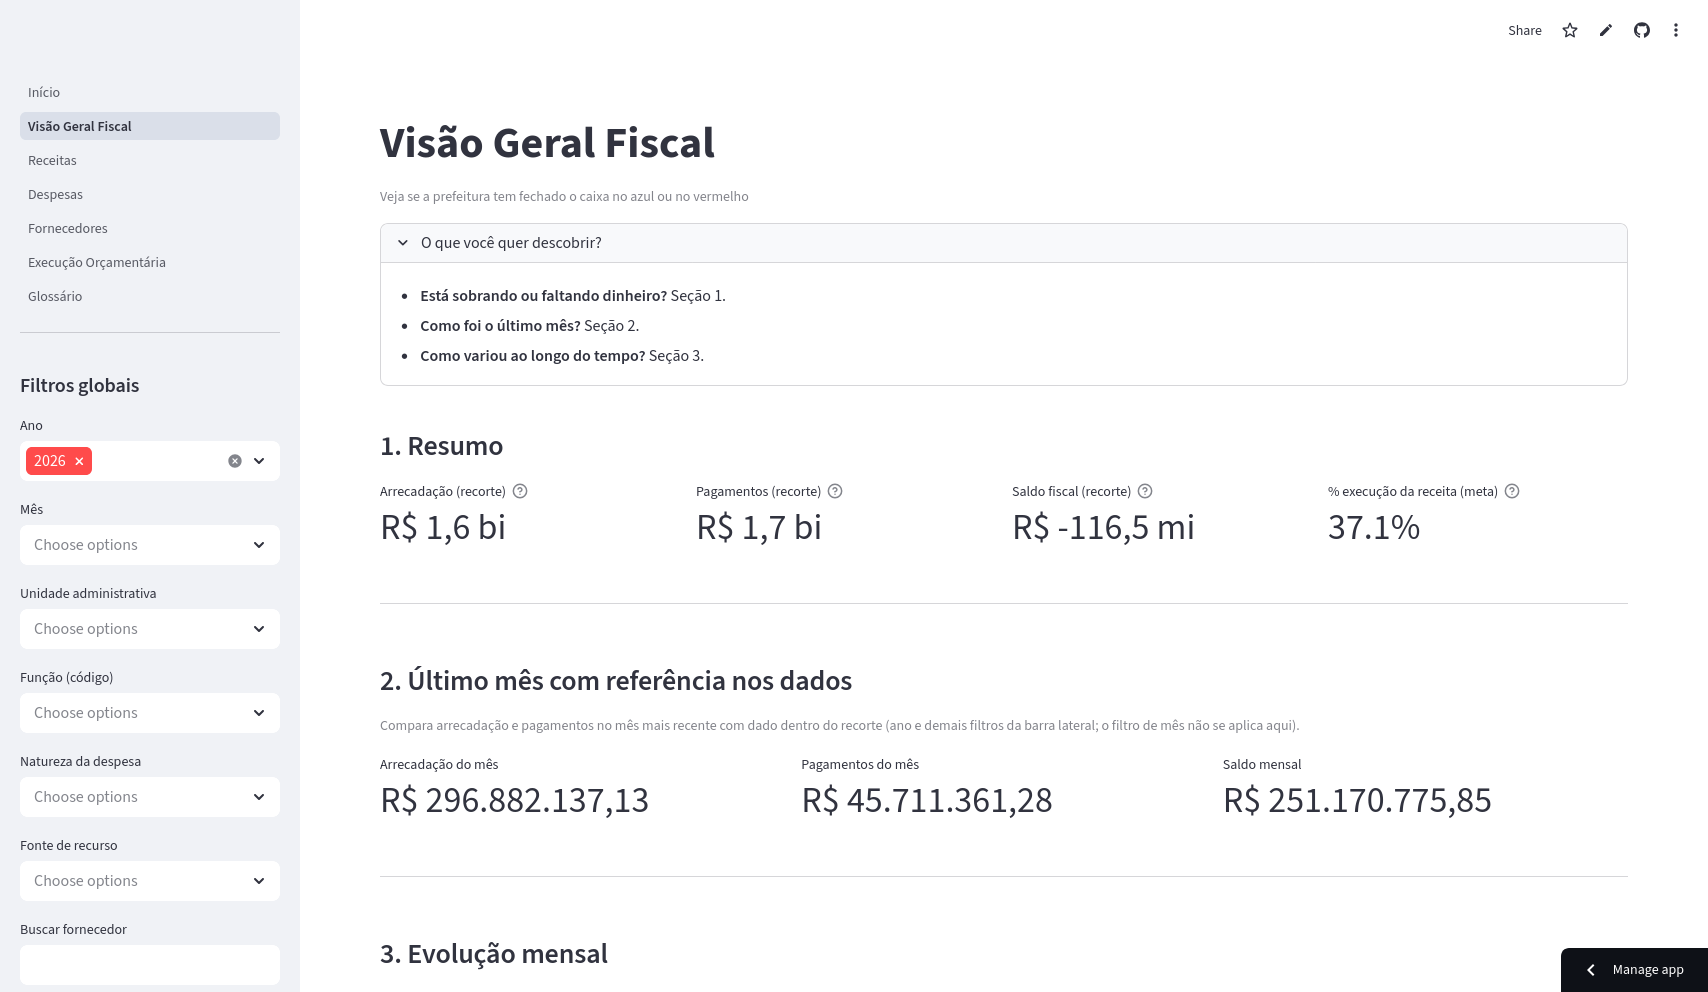
\includegraphics[width=\textwidth]{figs/visao_geral_fiscal_1_2.png}
\caption{Visão Geral Fiscal: resumo do recorte e comparação do último mês (seções 1 e 2).}
\label{fig:visao-geral-fiscal-resumo}
\end{center}
\end{figure}

\begin{figure}[h]
\begin{center}
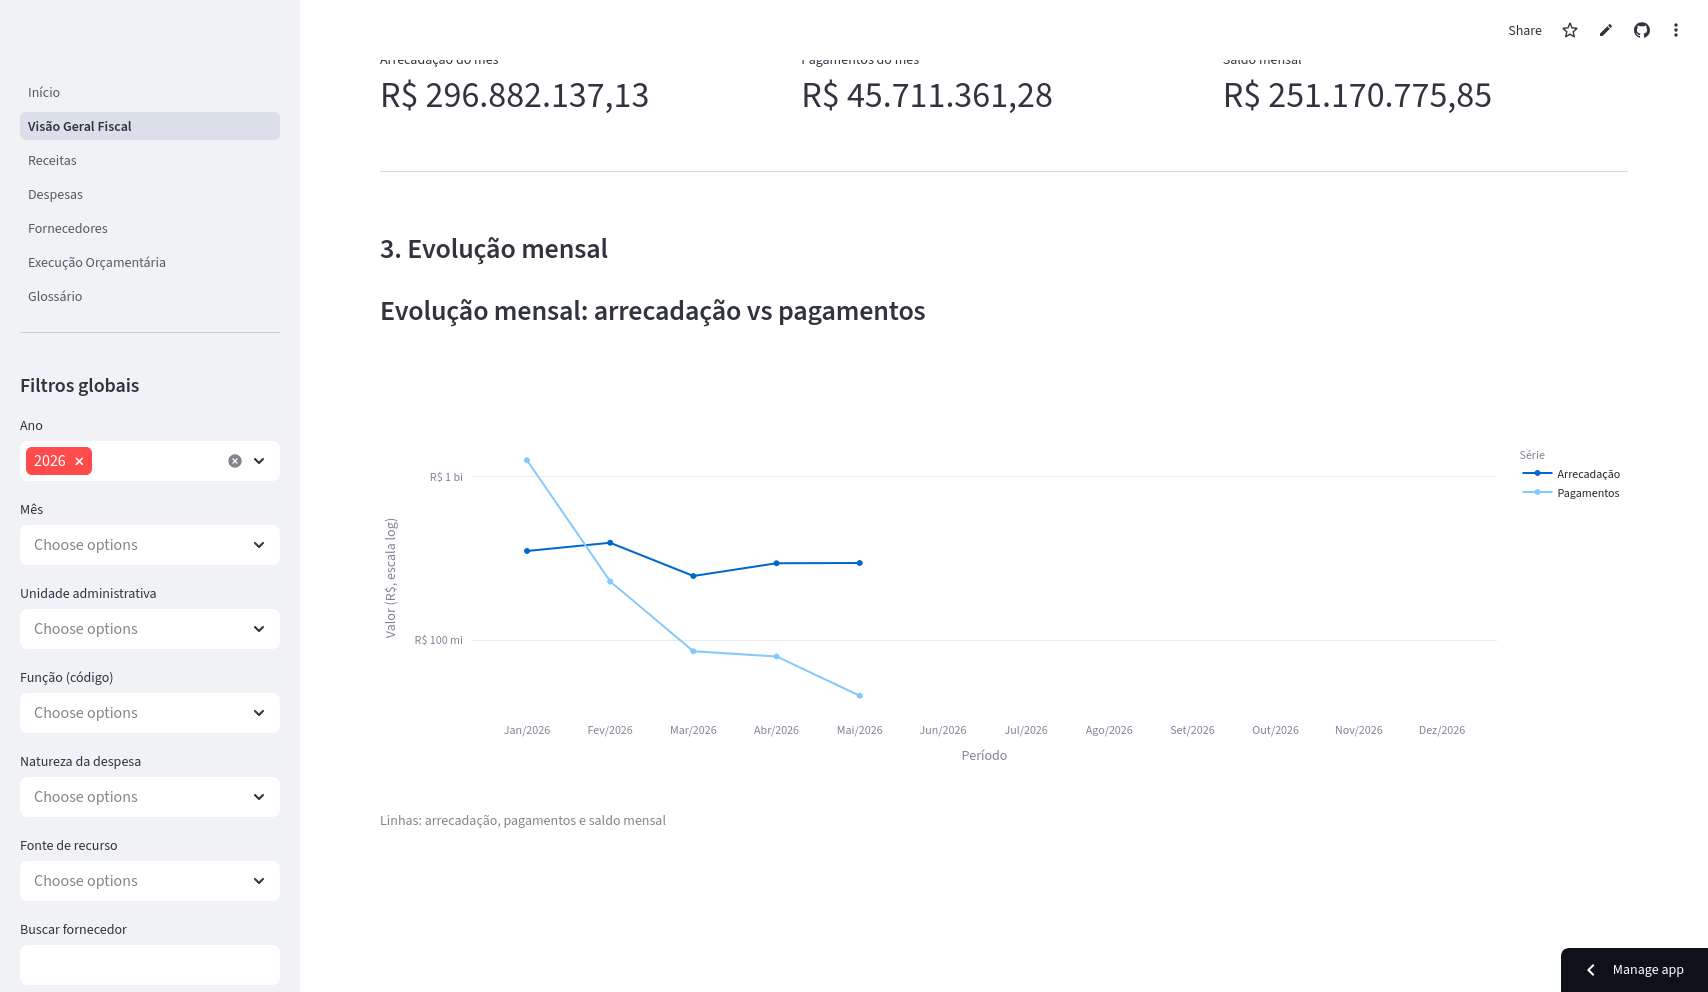
\includegraphics[width=\textwidth]{figs/visao_geral_fiscal_3.png}
\caption{Visão Geral Fiscal: evolução mensal de arrecadação \textit{vs.} pagamentos (seção 3).}
\label{fig:visao-geral-fiscal-evolucao}
\end{center}
\end{figure}

\begin{figure}[h]
\begin{center}
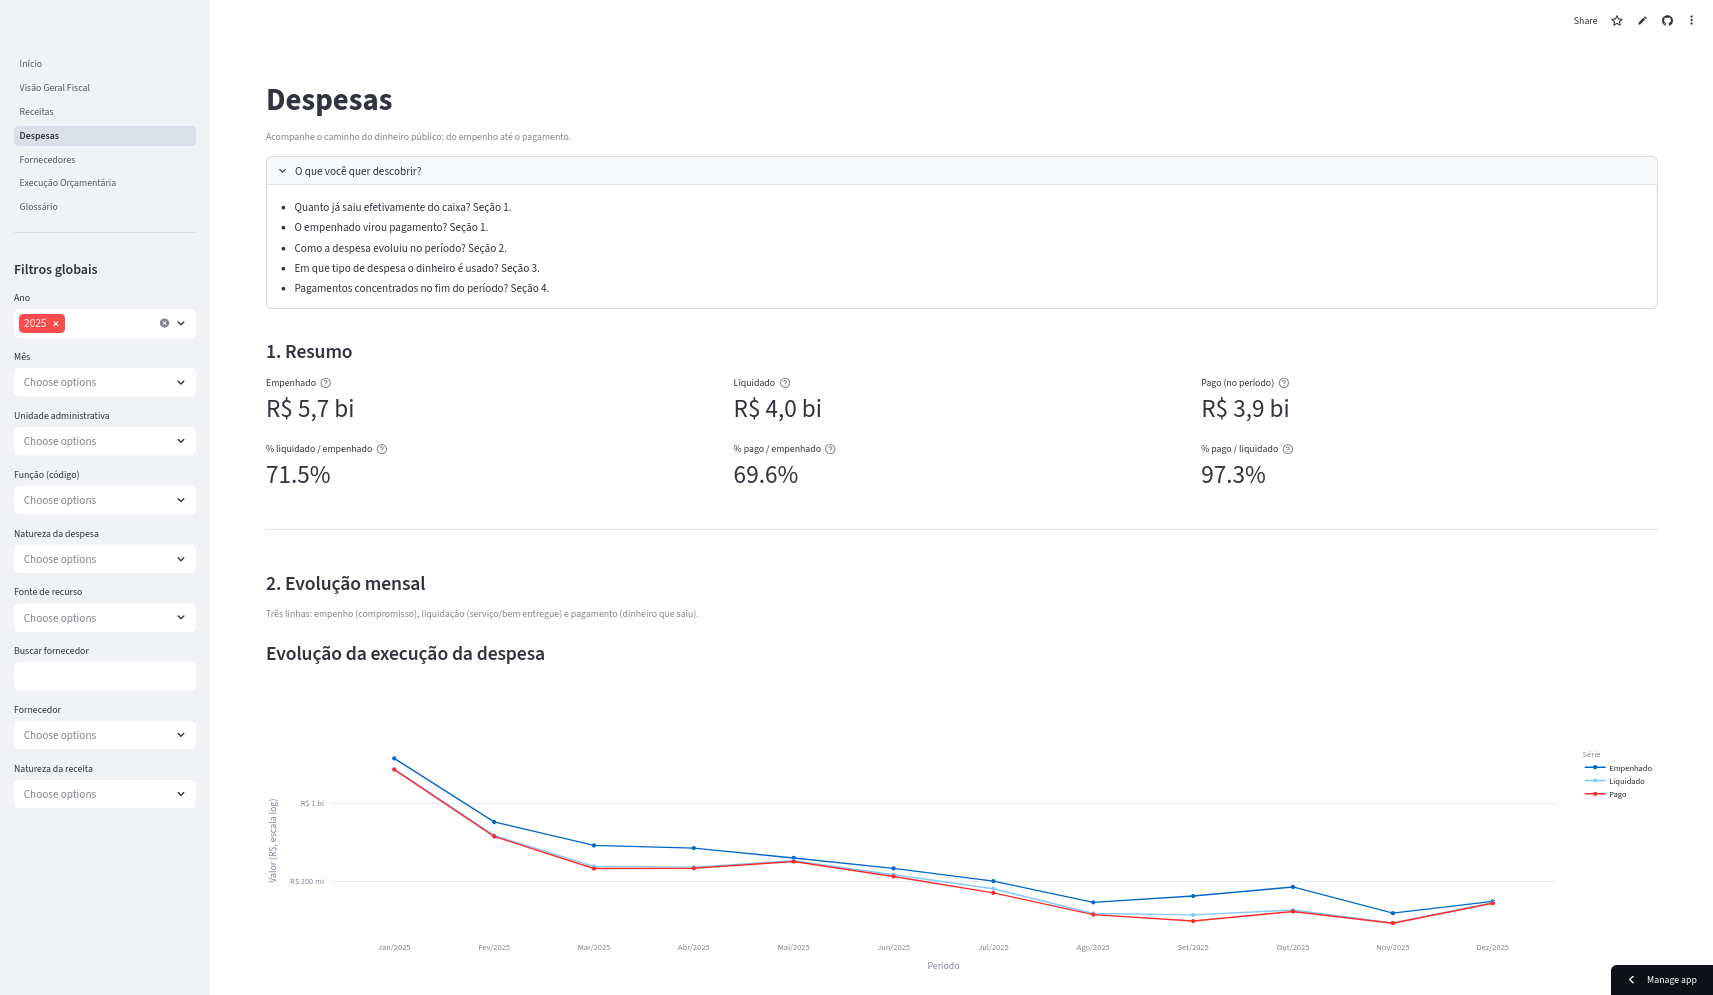
\includegraphics[width=\textwidth]{figs/despesas_1_2.png}
\caption{Despesas: resumo dos estágios da execução e da evolução mensal empenhada, liquidada e paga.}
\label{fig:despesas-resumo-evolucao}
\end{center}
\end{figure}

No portal municipal, receitas e despesas vivem em planilhas distintas, sem cruzamento automático nem série temporal unificada. Empenhado, liquidado e pago aparecem como colunas do relatório mensal, mas comparar estágios ao longo de anos ou filtrar por secretaria exige trabalho manual de consolidação. O painel reduz esse esforço a poucos cliques nos filtros globais e devolve, de imediato, indicadores que antes dependiam de uma planilha montada pelo próprio usuário.

\section{Execução por Função de Governo}

A página Execução Orçamentária desagrega a despesa por órgão executor e por classificação funcional. A primeira seção ordena as unidades administrativas pelos valores empenhados, liquidados e pagos no período, com um gráfico de barras agrupadas das vinte maiores e uma tabela completa ordenada por pagamento. A segunda seção extrai códigos de função e de subfunção da \textit{string} funcional programática publicada no consolidado mensal e faz \textit{join} com \texttt{dim\_funcao} e \texttt{dim\_subfuncao}, alimentadas pela LOA PJF do exercício 2026.

Essa página responde, com ressalvas, à pergunta exemplar da introdução: \textit{"Quanto Juiz de Fora investiu em educação nos últimos três anos?"}. Basta selecionar os anos desejados no filtro global e localizar, na tabela funcional, as linhas cuja função corresponde à educação. A comparação entre exercícios deixa de exigir abrir doze planilhas anuais e alinhar manualmente códigos funcionais programáticos.

\begin{figure}[h]
\begin{center}
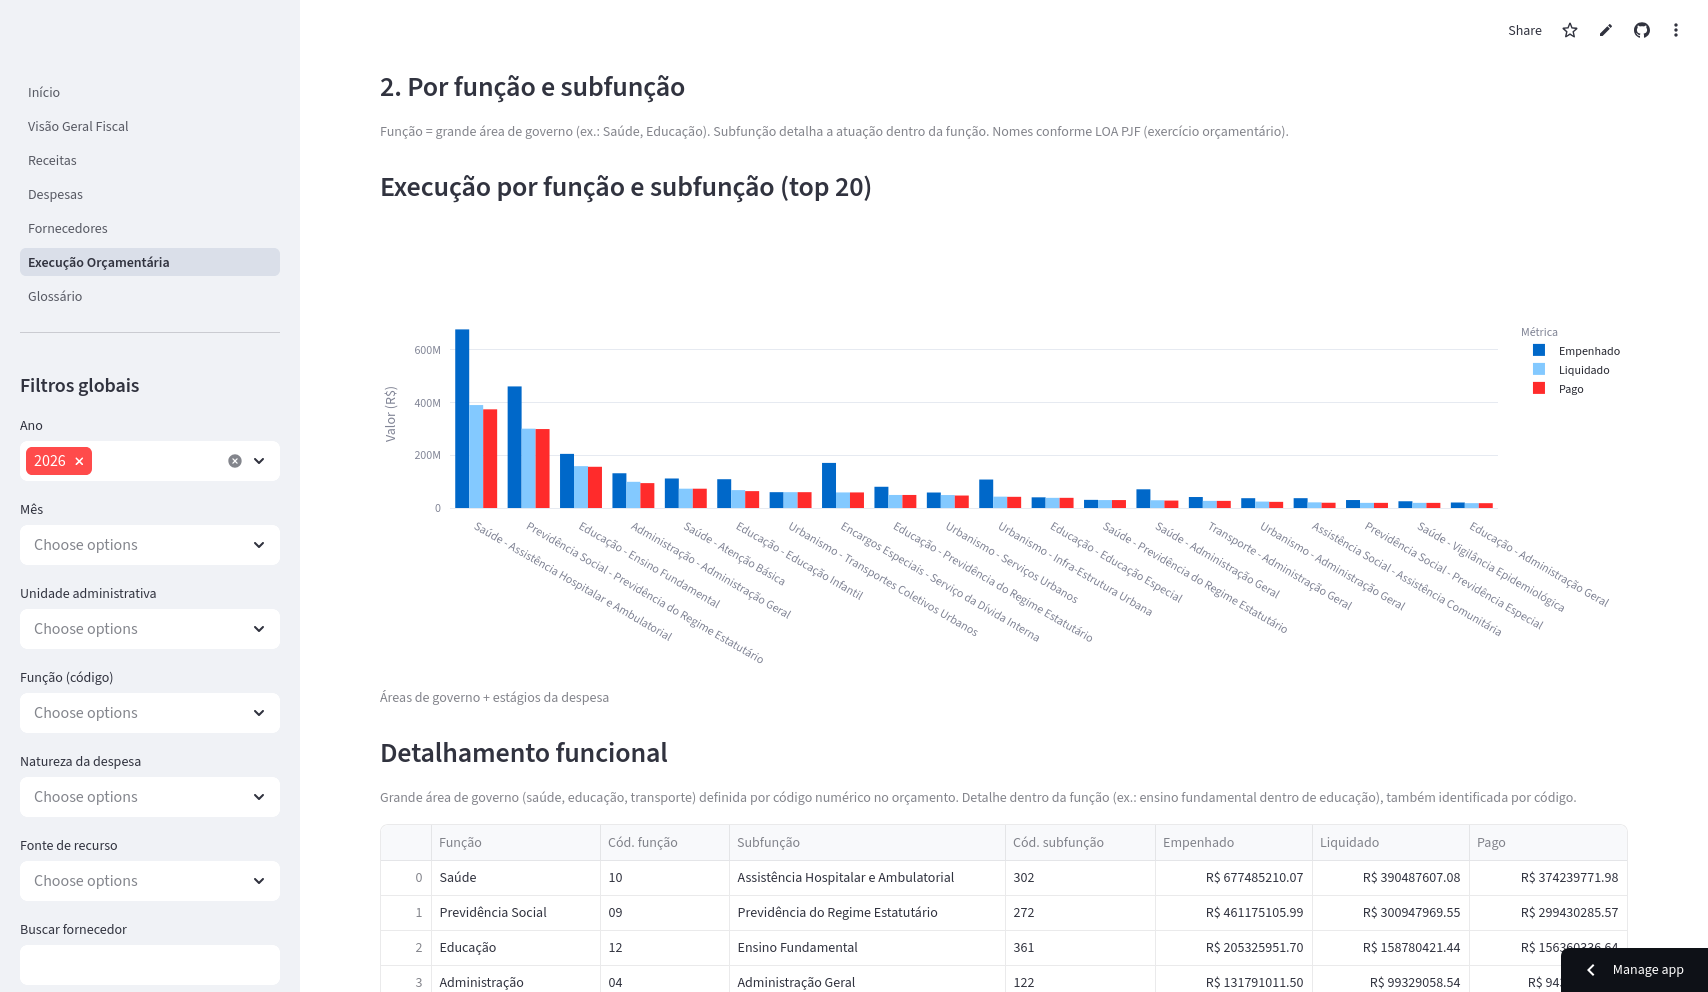
\includegraphics[width=\textwidth]{figs/exec_2.png}
\caption{Execução Orçamentária por função e subfunção: gráfico das vinte maiores combinações e tabela funcional.}
\label{fig:execucao-funcao}
\end{center}
\end{figure}

\section{Concentração de Fornecedores}

A página Fornecedores trata da questão do favorecimento e da concentração de recursos. O resumo destaca o maior favorecido do ranking, a base total de pagamentos considerada e a parcela acumulada pelos cinco primeiros do ranking. A seção de concentração exibe um gráfico horizontal com os vinte maiores pagamentos e uma tabela com valor pago, quantidade de empenhos distintos e participação percentual no total do recorte. A terceira seção permite escolher um fornecedor e visualizar a evolução mensal dos pagamentos a ele, o que é útil para verificar se um contrato pontual distorce o ranking ou se há recebimento recorrente ao longo do tempo.

O portal publica o favorecido e o valor pago na planilha de despesa, mas não calcula a participação relativa nem um ranking dinâmico filtrável por área ou período. Identificar concentração exige exportar, ordenar e normalizar manualmente, tarefa factível para, por exemplo, um jornalista, porém improvável para o cidadão sem intermediário. O indicador "\% nos 5 maiores" condensa essa análise em um número legível e convida à pergunta de fiscalização: a dependência de poucos credores é compatível com a natureza dos serviços contratados?

\begin{figure}[h]
\begin{center}
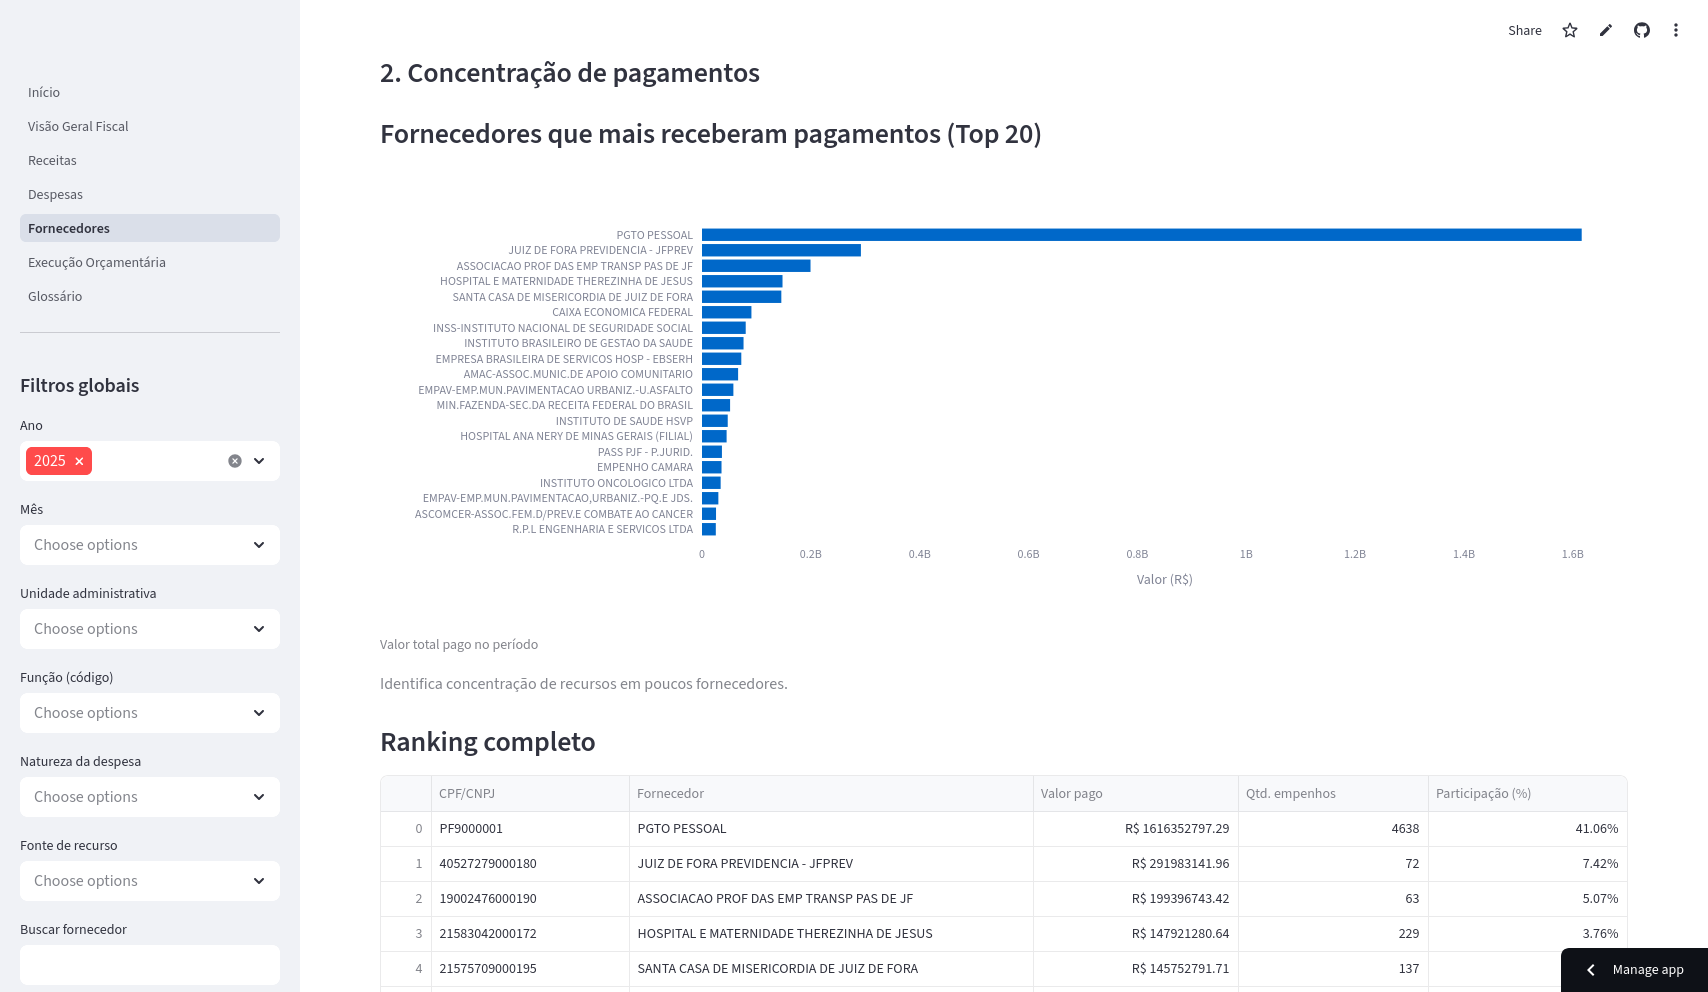
\includegraphics[width=\textwidth]{figs/fornecedores_concentracao.png}
\caption{Fornecedores: concentração de pagamentos (top 20) e ranking completo com participação percentual.}
\label{fig:fornecedores-concentracao}
\end{center}
\end{figure}

\section{Receitas Municipais}

A página Receitas organiza a entrada de recursos. O resumo contrasta previsão atualizada, arrecadação acumulada no recorte, razão realizado/previsão e parcelas classificadas como repasse federal e estadual, utilizando como base prefixos de natureza de receita. A seção "De onde vem o dinheiro" agrupa os códigos MCASP por origem interpretável e exibe barras horizontais por origem. Duas séries temporais comparam previsto e realizado: uma anual (ignorando o filtro de ano, mantendo mês e natureza) e outra mensal. A seção final "Previsto \textit{vs.} realizado" usa uma barra de progresso agregada e uma tabela por natureza de receita, com percentual de realização linha a linha.

Cruzar previsão e arrecadação no portal implica reconciliar arquivos comparativos e de previsão mensal, além de interpretar códigos de natureza sem ementário unificado. O \textit{warehouse} já integra descrições da STN quando disponíveis; o painel traduz a composição da receita em categorias próximas do debate público, o que aproxima o dado da pergunta "de onde vem o dinheiro da cidade?".

\begin{figure}[h]
\begin{center}
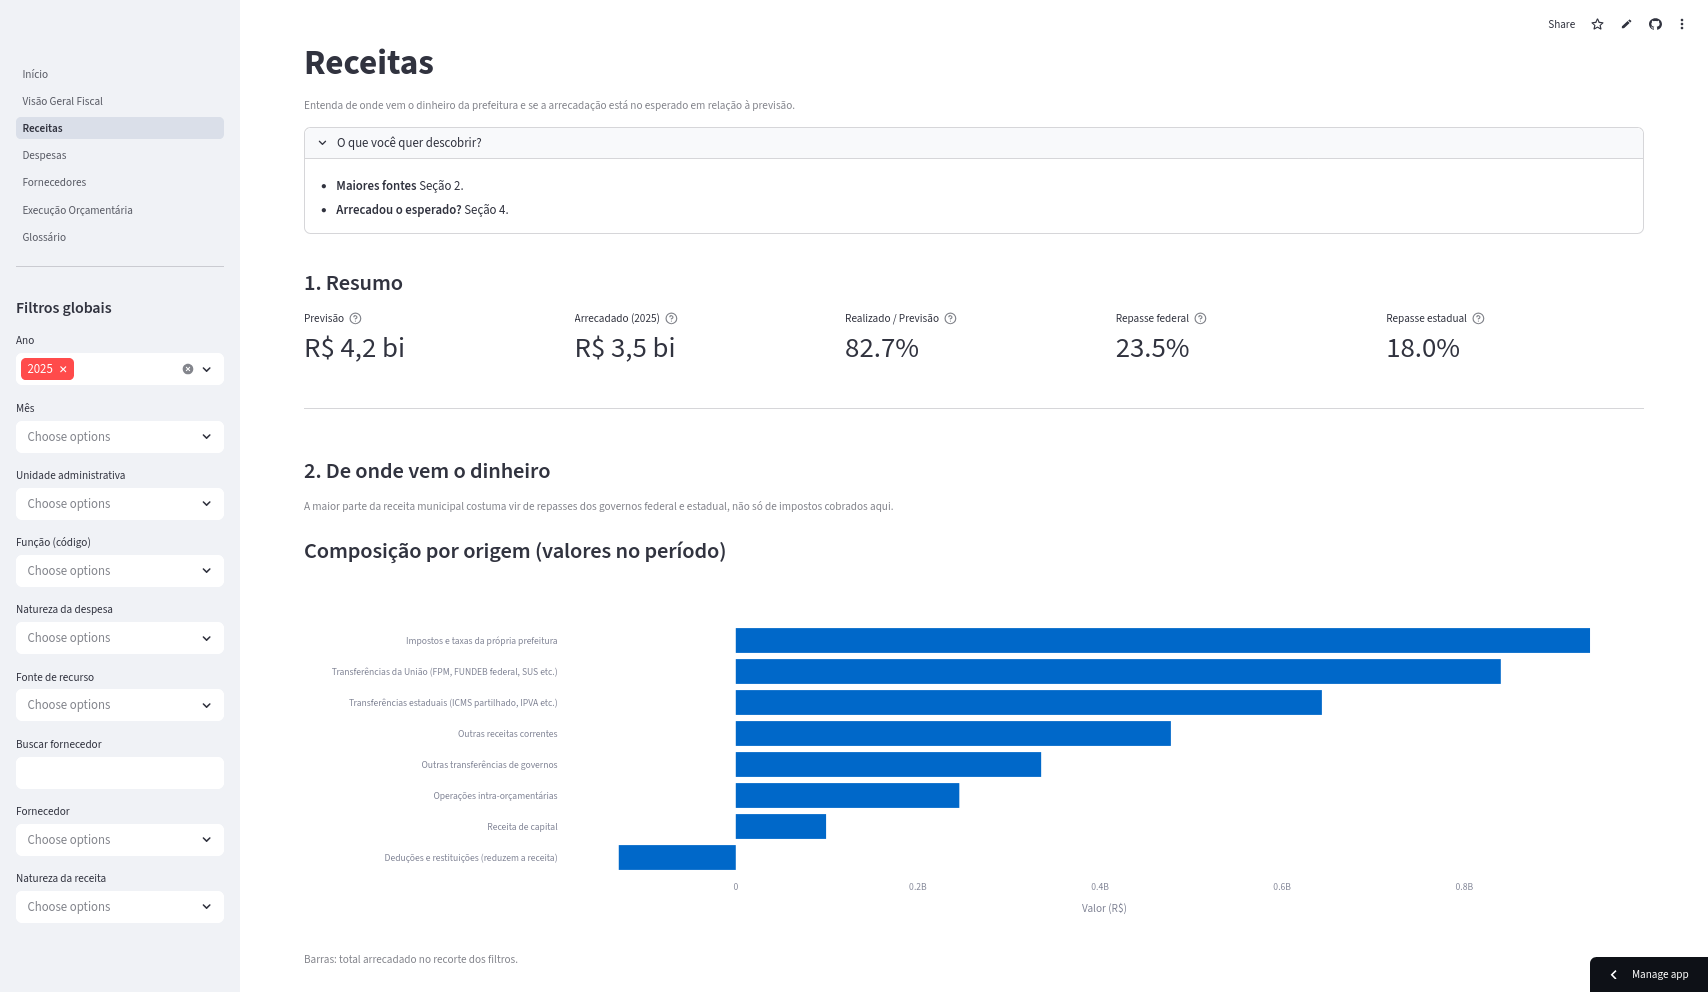
\includegraphics[width=\textwidth]{figs/receitas.png}
\caption{Receitas: resumo do recorte e composição por origem.}
\label{fig:receitas-origem}
\end{center}
\end{figure}

\section{Análise dos Dados de Juiz de Fora}

Descrever painéis não encerra o capítulo de resultados. A proposta do trabalho, ancorada na tradição freireana discutida no Capítulo~\ref{cap:fundamentacao}, exige ir além da descrição da interface e verificar o que o conjunto de números sugere ao ser lido pelo próprio artefato construído. Três padrões emergem da exploração sistemática do \textit{dashboard} sobre a base materializada.

\textbf{Dependência de transferências.} A composição por origem mostra, de forma recorrente, que transferências correntes respondem por parcela expressiva da arrecadação municipal. Isso não é específico de Juiz de Fora, mas torna visível uma premissa muitas vezes invisível no debate local: parte relevante do "orçamento da cidade" depende de repasses cujas regras são definidas fora do município. Um conselheiro ou vereador pode usar o painel para calibrar expectativas sobre o que a prefeitura controla diretamente \textit{vs.} o que é efeito de política nacional ou estadual.

\textbf{Distância entre empenho e pagamento.} Nas páginas de Despesas e Execução Orçamentária, o empenhado tende a superar o liquidado e pago no mesmo recorte quando o período inclui meses recentes do exercício. Isso reflete o ciclo contábil normal, mas também alerta contra leituras simplistas: "gastou" no sentido de empenho não coincide com "saiu do caixa". Restos a pagar e atrasos de liquidação só seriam mensuráveis com granularidade transacional ou com dotação autorizada, limitações já discutidas.

\textbf{Legibilidade funcional incompleta.} Os \textit{fallbacks} de rótulo LOA (Capítulo~\ref{cap:dw}) concentram-se em combinações de menor volume, mas ainda aparecem em cortes que um fiscalizador pode escolher deliberadamente. A análise cidadã ganha densidade quando o leitor combina a tabela funcional com o Glossário e, diante de \texttt{Função XX}, consulta o código ou busca esclarecimento junto ao órgão público.

O que um cidadão pode fazer com essa informação, além de informar-se? Formular perguntas para audiências públicas e sessões de câmara; subsidiar reportagens de jornalismo local com recortes exportáveis da tabela; apoiar entidades do controle social na escolha de prioridades de fiscalização. O painel não substitui um pedido formal de informação nem uma perícia contábil, mas reduz o custo para chegar à primeira evidência quantitativa, passo em que, no portal com dados brutos, muitas pessoas desistem de dar.

Os três padrões descritos acima ilustram o tipo de leitura que o painel viabiliza, mas não esgotam tudo o que ele permite. O Capítulo~\ref{cap:avaliacao} compara, de forma estruturada, o esforço necessário para realizar essas leituras no painel e no portal original.

\chapter{Avaliação e Discussão}
\label{cap:avaliacao}

Este capítulo confronta o que foi construído com o problema de pesquisa e com os objetivos declarados na introdução. A avaliação combina uma comparação estruturada entre o portal e o \textit{dashboard} com a discussão das limitações remanescentes e das implicações para a transparência e o controle social. Não houve teste de usabilidade com usuários finais, a avaliação aqui reportada é autoral, apoiada na reprodução repetida das mesmas perguntas nos dois ambientes.

\section{Avaliação da Usabilidade}

O critério de comparação adotado é funcional: "dada uma pergunta de fiscalização, o sistema permite respondê-la com quantos passos, em quanto tempo e com que grau de interpretação técnica intermediária?" Não se mede a estética da interface nem a satisfação subjetiva, o que se mede é a capacidade analítica relativa. A Tabela~\ref{tab:comparacao-portal-dashboard} resume seis tarefas representativas.

\begin{table}[htb]
\caption{Comparação portal PJF \textit{versus} \textit{dashboard} em tarefas de fiscalização}
\label{tab:comparacao-portal-dashboard}
\centering
\small
\renewcommand{\arraystretch}{1.5}
\begin{tabular*}{\textwidth}{@{\extracolsep{\fill}}p{4.2cm}p{4.8cm}p{4.8cm}@{}}
\hline
\textbf{Pergunta} & \textbf{Portal da Transparência} & \textbf{\textit{Dashboard}} \\
\hline
Saldo entre arrecadação e pagamentos no ano & Baixar planilhas de receita e despesa; alinhar competência; somar colunas manualmente & Página Visão Geral Fiscal; filtrar ano \\

Evolução mensal empenhado/liquidado/pago & Vários arquivos mensais; colar e consolidar & Página Despesas; gráfico único \\

Pagamentos por função & Filtrar planilha por código funcional; somar; decodificar código & Página Execução Orçamentária; filtrar anos; ler tabela com rótulos LOA \\

Participação dos maiores fornecedores & Exportar; ordenar; calcular \% no Excel & Página Fornecedores; indicador "\% nos 5 maiores" \\

Previsão \textit{vs.} arrecadação por natureza & Reconciliar comparativo e previsão; interpretar códigos & Página Receitas; tabela com \% de realização \\

Significado de "liquidação" & Buscar glossário externo ou norma & Glossário integrado + \textit{tooltips} \\
\hline
\end{tabular*}
\end{table}

Em todas as tarefas listadas, o portal contém a informação bruta, mas externaliza ao usuário o trabalho de integração. O \textit{dashboard} não cria novos dados: reorganiza o que já foi publicado e define convenções que, uma vez implementadas no \textit{warehouse}, não precisam ser refeitas a cada consulta. O ganho de usabilidade é, portanto, herdado da camada analítica descrita no Capítulo~\ref{cap:dw}, não de um truque de visualização isolado.

\section{Limitações do Trabalho}

As limitações do \textit{warehouse} (Capítulo~\ref{cap:dw}) propagam-se ao \textit{dashboard}. Ausência de dotação autorizada impede indicadores de execução sobre o previsto na LOA, métrica padrão em relatórios de controle interno. O grão por empenho existe no \textit{warehouse}, e \texttt{dim\_empenho} guarda a descrição e os metadados de licitação. O que falta é o detalhe abaixo do empenho. O pagamento aparece apenas como total mensal, sem data própria, o que dificulta a medição de prazos até a quitação. Itens, quantidades e preços de cada empenho não são publicados, e a interface ainda não usa esses metadados. Rótulos LOA com \textit{fallback} em cerca de 14\,\% dos pares função/subfunção presentes na execução comprometem a legibilidade pontual.

Limitações próprias da implementação do painel acrescentam-se às da fonte. O painel está publicado no \textit{Streamlit Community Cloud}\footnote{\url{https://juiz-de-fora-transparencia.streamlit.app/}}, lendo um DuckDB em arquivo empacotado na aplicação. O orquestrador Dagster, porém, não roda de forma agendada e, por isso, a atualização exige reexecutar manualmente o \textit{pipeline} e republicar o banco de dados. Os dados exibidos refletem, portanto, a última materialização, não necessariamente o portal em tempo real. Por fim, o cruzamento com licitações e contratos, citado na introdução como uma lacuna dos portais, permanece fora do escopo, embora conste como trabalho futuro.

\section{Implicações para Transparência e Controle Social}

Retomando as três lacunas da introdução, o sistema construído endereça cada uma delas em graus distintos.

A lacuna técnica é a mais diretamente atacada. Integrar receitas e despesas, conciliar planilhas heterogêneas, normalizar naturezas com o ementário STN e expor séries temporais filtráveis eliminam o gargalo de consolidação manual que a literatura associa aos portais municipais \cite{marco2022transparencia,melo2019proposta}. O cidadão deixa de depender de uma planilha intermediária montada por um especialista ao acessar o \textit{dashboard} em uma URL pública, sem instalar o ambiente localmente.

A lacuna social é parcialmente mitigada. Glossário, linguagem de "visão cidadã" e agrupamento das naturezas de receita por origem aproximam os termos do MCASP do vocabulário público. Permanecem os códigos nos filtros e a distância entre a classificação contábil e a experiência vivida: o painel mostra quanto foi pago em "saúde" na classificação funcional, não quanto foi investido em um equipamento específico no bairro do usuário. Transparência agregada educa sobre prioridades macro; não substitui prestação de contas situada.

A lacuna pedagógica encontra uma resposta incompleta. Freire \cite{freire1967liberdade} exige que o sujeito formule perguntas e construa interpretações, não apenas decodifique tabelas. Os \textit{expanders} orientadores, a estrutura por perguntas e a seção analítica do Capítulo~\ref{cap:resultados} empurram nessa direção. Kimball \cite{kimball2013data} fornece a estrutura orientada a assunto que torna a pergunta operacionalizável em SQL e, em seguida, em um gráfico. O encontro das duas tradições se materializa quando o usuário filtra por saúde, compara anos e questiona a concentração de fornecedores: gesto de "ler o mundo" orçamentário com ferramenta, não só para consumir um relatório passivo.

\section{Replicabilidade e Escalabilidade}

O modelo é replicável para outros municípios com portais que publiquem planilhas de execução em formato semelhante, mas a replicação não é uma cópia literal. Cada cidade impõe \textit{parsers} próprios. A arquitetura em camadas, extração com Dagster, \textit{staging} com dbt, \textit{warehouse} dimensional, consumo com Streamlit, permanece estável, o que muda são \textit{assets} de extração e dimensões auxiliares. Adaptar para vinte municípios mineiros exigiria, na prática, vinte conjuntos de regras de \textit{parsing} documentadas, preferencialmente com testes automatizados e política de manutenção quando os portais mudarem.

Escalar também é decisão institucional. Manter o \textit{pipeline} atualizado e o painel no ar exige uma rotina de \textit{backfill} e um responsável técnico, papel que, hoje, recai sobre o autor do TCC. A instância pública no \textit{Streamlit Community Cloud} reduz a barreira de acesso, mas não substitui a governança de dados nem o patrocínio institucional de longo prazo. Iniciativas \textit{civic tech} mostram impacto quando focadas \cite{marco2022transparencia}; sistemas institucionais duram mais, porém conservam recortes. Um meio-termo viável seria um observatório civil ou uma universidade local assumir a manutenção do \textit{pipeline} e da instância hospedada, com código aberto e documentação de reprodução já presentes no repositório do trabalho.

Para Juiz de Fora especificamente, o \textit{dashboard} já está disponível em uma URL pública. O próximo passo de maior retorno social seria automatizar a atualização do \textit{pipeline} e validar as tarefas da Tabela~\ref{tab:comparacao-portal-dashboard} com usuários reais. Sem essa cadência e sem evidência de uso pelo cidadão, a contribuição permanece uma ferramenta acessível, porém ainda pouco consolidada no debate democrático local.

\chapter{Conclusão}
\label{cap:conclusao}

\section{Síntese das Contribuições}

O trabalho propôs e implementou um Data Warehouse para a análise da execução orçamentária de Juiz de Fora, com o objetivo de tornar os dados públicos mais acessíveis e oferecer um modelo replicável para outros municípios.

O primeiro objetivo previa a coleta e documentação de dados de receitas e despesas do Portal da Transparência da Prefeitura. Foi atendido: o \textit{pipeline} de extração consome seis fontes (despesa mensal consolidada, receita mensal comparativa, receita mensal prevista, ementário de natureza de receita da STN, função LOA e subfunção LOA do exercício 2026), com tratamento explícito de heterogeneidades como mudança de \textit{layout} no meio do histórico, cabeçalho de planilha sem posição fixa e OCR nos PDFs da LOA.

O segundo objetivo, que previa a modelagem dimensional conforme o modelo de Kimball, foi cumprido. O \textit{warehouse} conta com dez dimensões e três tabelas de fatos organizadas em esquema de estrela compartilhando \texttt{dim\_tempo}. Cada decisão de granularidade foi escolhida em função do que a fonte de fato publica, sem inventar atomicidade que não está presente nos dados originais.

O terceiro objetivo previa a implementação de processos de ETL e foi atendido com Dagster como orquestrador, Python e \texttt{pandas} para extração, DuckDB como banco de dados analítico e dbt para modelagem em SQL. A unidade de idempotência foi definida como uma partição temporal, e três mecanismos garantem que a reexecução dessa mesma partição produza o mesmo estado final do \textit{warehouse}.

O quarto objetivo, que previa a construção de \textit{dashboards} interativos, também foi alcançado. Sete páginas em Streamlit consomem o \textit{warehouse}, estão publicadas em uma URL pública e respondem perguntas como a execução orçamentária por área, a evolução temporal de receitas, a concentração de fornecedores e o desvio entre previsão e arrecadação. A exploração sistemática descrita no Capítulo~\ref{cap:resultados} destacou duas leituras recorrentes: dependência de transferências intergovernamentais na arrecadação e a distância entre empenho e pagamento ao longo do exercício.

Complementarmente, o Capítulo~\ref{cap:avaliacao} compara o portal e o \textit{dashboard} em seis tarefas de fiscalização. O painel reduz os passos manuais de consolidação em todas elas. A lacuna técnica dos portais foi a mais atendida, e a pedagógica, parcialmente.

\section{Considerações Finais}

O processo de construção deste \textit{warehouse} revelou algo que não estava previsto no plano inicial. O problema central da transparência orçamentária municipal não é técnico no sentido mais estreito da palavra.

O problema está na distância entre o que o portal publica e o que o cidadão precisa para fiscalizar. O portal publica relatórios mensais consolidados em planilhas Excel. O cidadão precisa de séries temporais comparáveis, classificações inteligíveis e indicadores que dialoguem com sua experiência cotidiana. Reduzir essa distância é trabalho de arquitetura de dados, e arquitetura de dados é, em última análise, uma decisão sobre quem deve interpretar a informação pública. Quando se publica o valor apenas em colunas mensais, sem a data de cada pagamento e sem abrir o empenho por itens, decide-se o que o cidadão pode ver. Ele enxerga quanto saiu no mês e a descrição do empenho. Não enxerga o ritmo dos pagamentos, nem a quantidade nem o preço do que foi comprado.

A leitura freireana ganha contorno técnico nesse ponto. Conscientização orçamentária, traduzida para o trabalho de quem constrói \textit{data warehouses}, significa modelar o dado pensando em quem vai lê-lo, e não apenas em quem vai gerá-lo.

\section{Trabalhos Futuros}

A continuação natural do trabalho segue cinco direções concretas:

(1) Integração da dotação autorizada pela LOA, viabilizando indicadores percentuais de execução sobre o autorizado, que são a métrica padrão utilizada por órgãos de controle. A classificação funcional do exercício de 2026 já está no DW.

(2) Desagregação da funcional programática em programa e ação, com \textit{parsers} LOA adaptados a exercícios anteriores e, se necessário, aos ementários oficiais da STN para níveis ainda ausentes.

(3) Captura de licitações e contratos como processos de negócio adicionais, permitindo rastrear a cadeia completa do gasto e analisar o tempo médio entre as etapas.

(4) Implementação de SCDs do tipo 2 nas dimensões sujeitas a mudanças históricas, permitindo análises "como era" \textit{vs.} "como é".

(5) Replicação do modelo em pelo menos um município de porte semelhante, com análise comparativa, para validar a generalidade do esquema dimensional proposto e identificar pontos de adaptação locais.

Cada uma dessas direções é viável com o ferramental atual e não exige reescrita das camadas já implementadas. O DW aqui construído, quando tomado em conjunto com a discussão teórica que o sustenta, não esgota o problema da transparência orçamentária. Oferece, em vez disso, uma peça de evidência de que é possível, no escopo de um trabalho, trilhar o caminho entre o dado bruto que a prefeitura publica e a pergunta que o cidadão de fato faria. Essa ponte é a contribuição.


% -----Bibliografia---------------------------------
\singlespacing
\bibliographystyle{abntex2-alf}
\bibliography{referencias}

% --------------------------------------------------
\end{document}
